\documentclass[10pt,a4paper]{article}

\usepackage[T1]{fontenc}
\usepackage[utf8]{inputenc}
\usepackage{lmodern}
\usepackage[margin=2.3cm]{geometry}
\usepackage{microtype}
\usepackage{amsmath,amssymb}
\usepackage{graphicx}
\usepackage{booktabs}
\usepackage{tabularx}
\usepackage{array}
\usepackage{longtable}
\usepackage{xcolor}
\usepackage{caption}
\usepackage{subcaption}
\usepackage{url}
\usepackage{placeins}
\usepackage[numbers,sort&compress]{natbib}
\usepackage{tikz}
\usetikzlibrary{positioning,arrows.meta,fit,backgrounds}
\usepackage[colorlinks=true,linkcolor=blue!50!black,citecolor=blue!50!black,urlcolor=blue!50!black]{hyperref}

\captionsetup{font=small,labelfont=bf,margin=0.5em}
\setlength{\parskip}{0.35em}
\renewcommand{\arraystretch}{1.12}
\newcolumntype{L}{>{\raggedright\arraybackslash}X}
\newcommand{\seg}[1]{\texttt{#1}}
\newcommand{\hyp}[1]{\textsf{#1}}

\title{\textbf{AI\_Trader: building a forward-only trading system\\with an LLM as the decision layer}\\[0.4em]
\large Methodology, models, results and lessons from the first nine days (2026-11-07 to 2026-11-15)}
\author{The AI\_Trader project\\[0.2em]\small Written with Claude (model \texttt{claude-opus-5-5}) from the project's research record}
\date{15 November 2026}

\begin{document}
\maketitle

\begin{abstract}
\noindent
AI\_Trader is a research system for trading Bybit USDT linear perpetuals in which a large language model (Claude) is the decision-maker, but never the source of numbers. Because an LLM is non-deterministic and has read about every period before its training cutoff, its decisions cannot be backtested; the system is therefore split into a deterministic layer (data, tools, screener, risk engine), which is validated historically, and a judgment layer, which is measured only forward against paired baselines on the same candidate list. Every historical result is reported twice, before and after the model's knowledge cutoff of 2026-07-01 (\seg{llm\_in\_sample} and \seg{clean\_holdout}). In nine days the project registered 252 hypotheses before testing them and recorded 442 results; 33 hypotheses are supported in both segments, 90 are refuted and 26 flip sign across the cutoff. Our own priors averaged 0.44 while only 22\% of decided hypotheses held up. The robust findings are about volatility, not direction: log-HAR and small neural networks forecast variance well, the calendar (weekends, hour of week) explains most of the nonlinear gain, and every direction test sits at coin-flip level. The only execution edge measured so far is small: limit entries at the touch beat market entries by $+0.010$\,R per signal. A probability field fitted by sparse Kramers--Moyal regression, a Kolmogorov--Arnold-style polynomial-neuron network with adaptive conformal bands, a 23-token cross-sectional network and a Bybit-semantics matching engine were built and tested; each beats a simple baseline at short horizons for variance, and none adds a tradable directional signal. The live hourly network, Claude's interpreted forecasts and a paper decision book are now accruing forward evidence; the first paper trade lost $-1.28$\,R. We describe the rules, the models, the results, the expected sources of P\&L, the falsification tests and the mistakes made along the way.
\end{abstract}


%=====================================================================================================
\section{Introduction and design principles}
%=====================================================================================================

The project starts from a constraint, not a strategy. The decision-maker is Claude, and an LLM has two properties that make a backtest of its decisions meaningless (\protect\path{docs/PLAN.md}, \S1). It is \emph{non-deterministic}: the same inputs can give different decisions, so a historical run cannot be reproduced. And it is \emph{contaminated by its training data}: for any date before its knowledge cutoff the model has read what happened next, so even masked or anonymised backtests carry look-ahead bias \citep{glasserman2023,sarkar2024,lopezlira2023}. The consequence is the first non-negotiable principle of the repository (\protect\path{CLAUDE.md}): \emph{the LLM decision layer is never backtested}. Its performance is measured only forward, after the cutoff, against paired baselines that trade the same candidate list under the same risk engine.

Everything else must then be deterministic and historically testable. The system is organised in five layers (Table~\ref{tab:layers}); the LLM interprets numbers that the tools compute, and it never sizes a position or overrides a risk limit.

\begin{table}[h]
\centering\small
\begin{tabularx}{\textwidth}{@{}l L l@{}}
\toprule
Layer & What it is & Backtestable? \\
\midrule
Data & Point-in-time market and alternative data; every record carries \texttt{event\_ts} and \texttt{known\_ts} & yes \\
Tools & Deterministic functions: volatility, regimes, levels, flow, forecasts, screeners & yes, and they must be validated \\
Judgment & Claude reads tool outputs, forms a view, takes or skips candidates & no: forward only \\
Risk and execution & Fixed risk per trade, caps, stops, sizing, order routing (Rust) & yes, as deterministic replay \\
Journal and evaluation & Every prompt, tool call, decision and fill; paired scorecards & n/a \\
\bottomrule
\end{tabularx}
\caption{The layer split (\protect\path{docs/PLAN.md}, \S2).}
\label{tab:layers}
\end{table}

Eight principles in \protect\path{CLAUDE.md} govern all work. (1) The LLM layer is forward-only. (2) Everything else is deterministic and must be testable historically. (3) Point-in-time everything: every data and tool call takes an \texttt{as\_of} argument, and returning data stamped after \texttt{as\_of} is a bug; the lake enforces it with a bitemporal schema in which every read is \texttt{WHERE known\_ts <= :as\_of} (\protect\path{docs/ARCHITECTURE.md}, \S6.2). (4) The LLM interprets but does not compute or size; position size comes from the risk engine at a fixed risk per trade. (5) Statistical house rules (\protect\path{docs/ARCHITECTURE.md}, \S1): log returns, volatility-standardised features $z_t = r_t/\hat\sigma_{t|t-1}$, Student-$t$ errors by default, ADF and KPSS stationarity checks, heteroskedasticity- and autocorrelation-consistent standard errors \citep{neweywest1987} clustered by time because crypto moves together, purged walk-forward validation, calibrated probabilities and a linear-first complexity budget. (6) A research protocol with pre-registration. (7) A diary that is never edited after the fact. (8) Pinning and logging: model ID, prompt version and tool versions are logged per session, and changing any of them starts a new track record.

\paragraph{The cutoff split.} The protocol (\protect\path{docs/RESEARCH_PROTOCOL.md}) extends the contamination argument to research itself: the \emph{ideas} Claude proposes are shaped by papers and forum lore about the very periods being tested, so an in-sample ``discovery'' may be recall. Every result is therefore reported in two segments split at \texttt{research.knowledge\_cutoff} $=$ 2026-07-01. The \seg{llm\_in\_sample} segment (before the cutoff) is weak, necessary-but-not-sufficient evidence; the \seg{clean\_holdout} segment (after it, about 135 days at the time of writing) is strong evidence that grows every day. A hypothesis is \emph{supported} only if it holds in-sample \emph{and} keeps its sign in the holdout. The holdout is read once per registered hypothesis; a holdout used for selection is in-sample.

%=====================================================================================================
\section{System architecture}
%=====================================================================================================

The language split follows one rule: Rust for anything always-on, per-bar or touching money; Python for fitting, research, point-in-time reads and LLM orchestration (``fit in Python, filter in Rust'', with parameters handed over as JSON under \protect\path{data/models/}). Figure~\ref{fig:arch} shows the data path from the exchanges to the journal.

\begin{figure}[t]
\centering
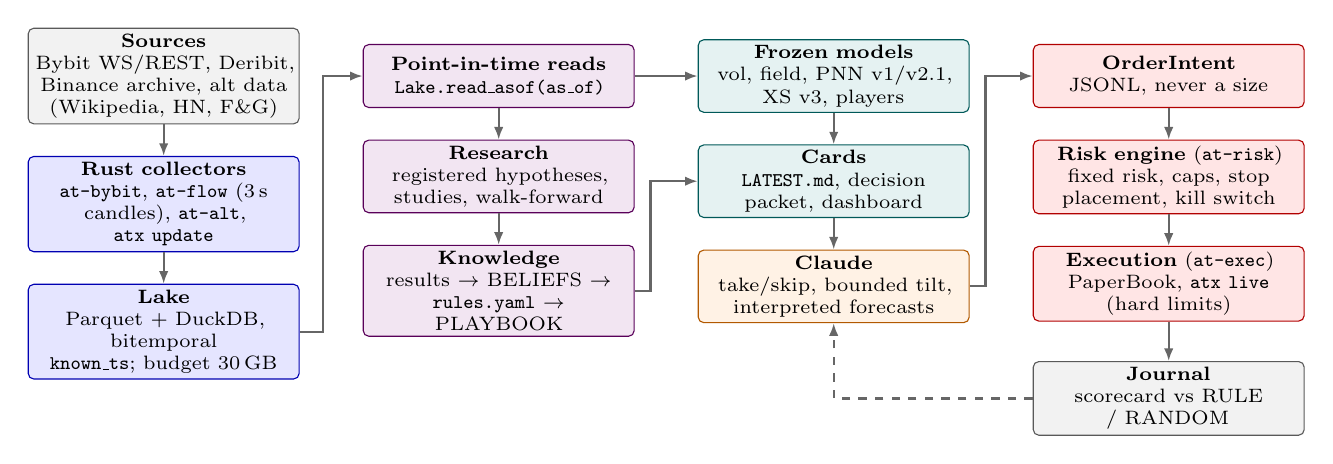
\begin{tikzpicture}[
  font=\scriptsize, node distance=4mm and 5mm,
  box/.style={draw=#1!70!black, fill=#1!10, rounded corners=2pt, align=center, minimum height=8mm, text width=33mm, inner sep=2pt},
  arr/.style={-{Latex[length=1.6mm]}, thick, draw=black!60}]
% column 1: sources and collectors
\node[box=gray] (src) {\textbf{Sources}\\Bybit WS/REST, Deribit,\\Binance archive, alt data\\(Wikipedia, HN, F\&G)};
\node[box=blue, below=of src] (coll) {\textbf{Rust collectors}\\\texttt{at-bybit}, \texttt{at-flow} (3\,s\\candles), \texttt{at-alt}, \texttt{atx update}};
\node[box=blue, below=of coll] (lake) {\textbf{Lake}\\Parquet + DuckDB, bitemporal\\\texttt{known\_ts}; budget 30\,GB};
% column 2: research
\node[box=violet, right=8mm of src] (read) {\textbf{Point-in-time reads}\\\texttt{Lake.read\_asof(as\_of)}};
\node[box=violet, below=of read] (stud) {\textbf{Research}\\registered hypotheses,\\studies, walk-forward};
\node[box=violet, below=of stud] (know) {\textbf{Knowledge}\\results $\to$ BELIEFS $\to$\\\texttt{rules.yaml} $\to$ PLAYBOOK};
% column 3: models and LLM
\node[box=teal, right=8mm of read] (models) {\textbf{Frozen models}\\vol, field, PNN v1/v2.1,\\XS v3, players};
\node[box=teal, below=of models] (card) {\textbf{Cards}\\\texttt{LATEST.md}, decision\\packet, dashboard};
\node[box=orange, below=of card] (llm) {\textbf{Claude}\\take/skip, bounded tilt,\\interpreted forecasts};
% column 4: risk and execution
\node[box=red, right=8mm of models] (intent) {\textbf{OrderIntent}\\JSONL, never a size};
\node[box=red, below=of intent] (risk) {\textbf{Risk engine} (\texttt{at-risk})\\fixed risk, caps, stop\\placement, kill switch};
\node[box=red, below=of risk] (exec) {\textbf{Execution} (\texttt{at-exec})\\PaperBook, \texttt{atx live}\\(hard limits)};
\node[box=gray, below=5mm of exec] (journal) {\textbf{Journal}\\scorecard vs RULE / RANDOM};
\draw[arr] (src) -- (coll); \draw[arr] (coll) -- (lake);
\draw[arr] (lake.east) -- ++(3mm,0) |- (read.west);
\draw[arr] (read) -- (stud); \draw[arr] (stud) -- (know);
\draw[arr] (read) -- (models); \draw[arr] (models) -- (card); \draw[arr] (card) -- (llm);
\draw[arr] (know.east) -- ++(2mm,0) |- (card.west);
\draw[arr] (llm.east) -- ++(2mm,0) |- (intent.west);
\draw[arr] (intent) -- (risk); \draw[arr] (risk) -- (exec); \draw[arr] (exec) -- (journal);
\draw[arr, dashed] (journal.west) -| (llm.south);
\end{tikzpicture}
\caption{System architecture. Blue: Rust ingestion and storage. Violet: Python research and the knowledge pipeline. Teal: frozen deterministic models and the cards Claude reads. Orange: the only non-deterministic component. Red: the deterministic Rust risk and execution path, which never takes a size from the LLM.}
\label{fig:arch}
\end{figure}

\paragraph{Data and the lake.} The universe is Bybit USDT linear perpetuals: a research universe L of 23 liquid crypto perps, plus 16 TradFi perps (equity, index and commodity perps that Bybit lists) used as context and for robustness. Bars, funding and open interest are stored as Parquet (zstd, \texttt{float32}) queried in-process by DuckDB; there is no database server. The schema in \protect\path{config/schema.yaml} is shared by Rust and Python. Every table carries \texttt{event\_ts} and \texttt{known\_ts}; revisions are new rows, never in-place updates. Order flow is stored only as 3-second candles (\texttt{flow\_3s}); one-minute rollups and moving-average stacks are derived (\protect\path{docs/ORDER_FLOW.md}). The collector went live on 2026-11-07 with 70 streams (48 linear perps, 20 spot) at about 59 bytes per candle, which fits roughly 200 days of 3-second data into the 30\,GB lake budget; it grew to 124 streams the next day. Liquidations have been collected since 2026-11-08 00:43 UTC. The collector runs from a copy of the binary so that rebuilds never hit a locked executable.

\paragraph{Risk engine.} The Rust crate \texttt{at-risk} receives an \texttt{OrderIntent} (symbol, side, entry, stop, targets, volatility forecasts, the rules applied by the bias gate) and returns a \texttt{RiskDecision} with a quantity and the list of named rejections (\protect\path{docs/EXECUTION_PIPELINE.md}). An intent never carries a size. The paper profile in \protect\path{config/risk.yaml} risks 0.5\% of equity per trade (fees and slippage included), allows at most 3 new trades per UTC day, 5 open positions, one position per strategy-family cluster (the book is about one trend bet, Section~\ref{sec:results}), a 1.5\% daily loss limit, 3$\times$ gross exposure, and a minimum net expected value of 0.10\,R after costs (relaxed to $>0$ for paper and replay only, by an explicit operator decision on 2026-11-14). Stops are placed between minimum and maximum distances in units of the unshrunk risk sigma. A file flag \protect\path{data/exec/KILL} cancels and flattens.

\paragraph{Paper and live pipeline.} Strategies emit point-in-time signals; a Python bias gate applies the machine-checkable rules of the playbook (for example: never fade a 2-sigma hourly move; no 1-hour mean reversion in trend cells) and writes intents; \texttt{atx exec-intents} sizes them in Rust and drives \texttt{at-exec}'s PaperBook (stop first when both stop and target are touched in one bar). The decision harness \protect\path{src/ai_trader/agent/decision.py} runs Claude every four hours on this book (Section~\ref{sec:live}). A separate live profile, \texttt{live\_small}, was added on 2026-11-15 (Section~\ref{sec:live}).

\begin{figure}[t]
\centering
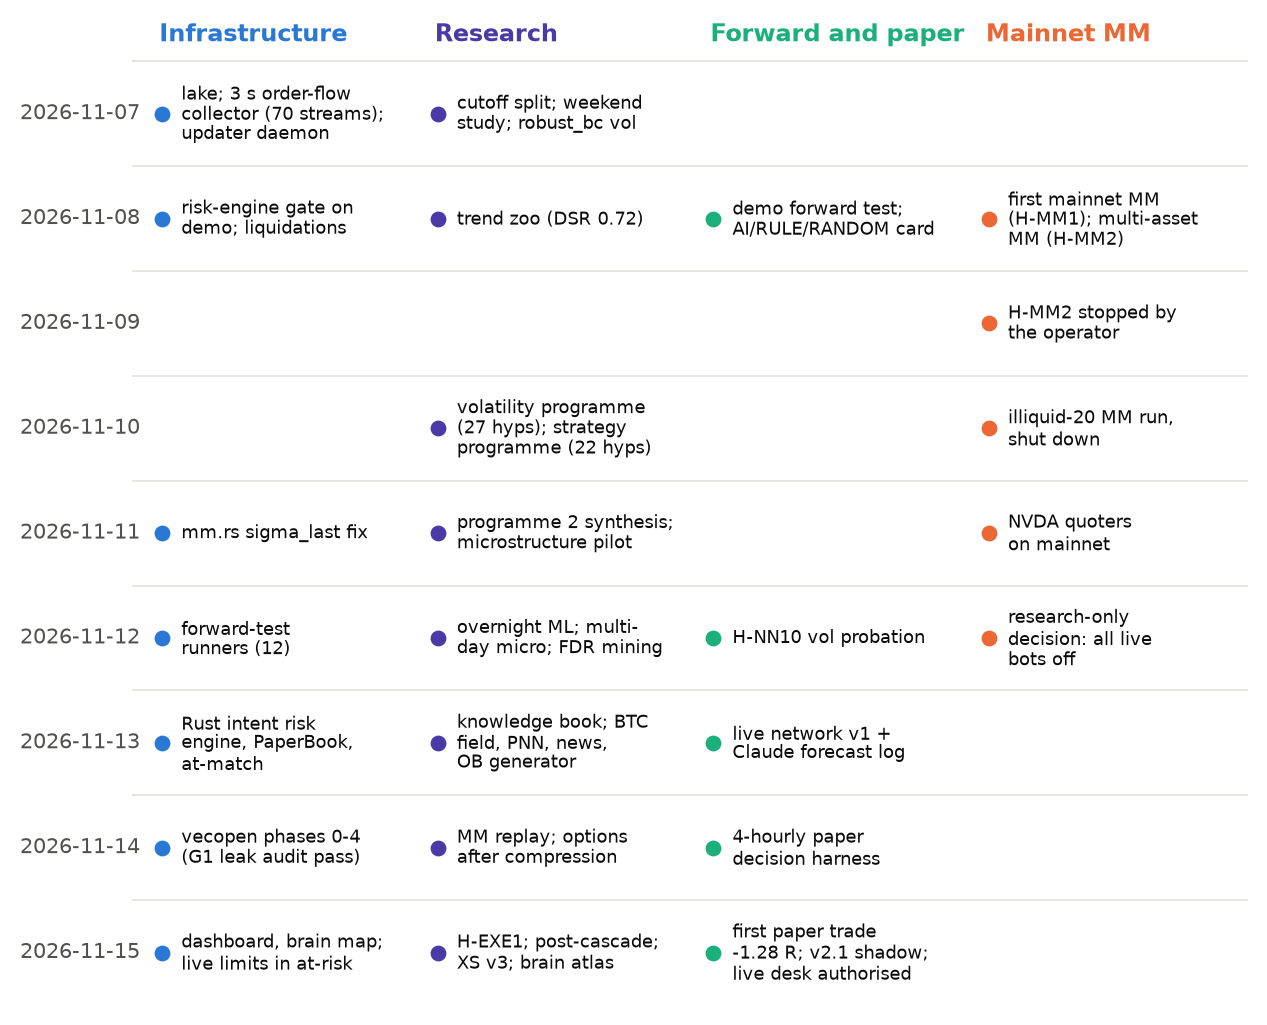
\includegraphics[width=0.8\textwidth]{figures/timeline.png}
\caption{Timeline of the build, from the research diary (\protect\path{research/diary/2026-11-07.md} to \protect\path{2026-11-15.md}).}
\label{fig:timeline}
\end{figure}

%=====================================================================================================
\section{Research protocol and the knowledge pipeline}
%=====================================================================================================

\subsection{From hypothesis to rule}

Each idea follows the same lifecycle (\protect\path{docs/RESEARCH_PROTOCOL.md}, \S2). It is first registered in \protect\path{research/hypotheses.yaml} with a statement, rationale, test, success criterion, family and a subjective prior probability, \emph{before} any result is seen. It is then tested with deterministic code and recorded, success or failure, as an append-only line in \protect\path{research/hypotheses_results.jsonl} with its segment, verdict and metrics. Changing a hypothesis after seeing results means registering a new identifier (for example \hyp{H-W5b} after \hyp{H-W5}) and counting it as an additional trial. Anything chosen from more than five variants is deflated \citep{bailey2014dsr}; selection overfitting is measured with the probability of backtest overfitting \citep{bailey2017pbo}; families of tests are Holm-adjusted \citep{holm1979}. Signals are computed on the full history and the P\&L is then split by segment, so indicator warm-up never empties the holdout.

Supported results are compressed into the working beliefs of \protect\path{research/BELIEFS.md} (graded A: both segments and a large effect; B: a small effect or confirmed once; C: plausible, forward test running) and then into decision rules in \protect\path{research/rules.yaml}. A rule has a fixed schema: an identifier, a kind (\emph{expect}, \emph{prefer} or \emph{avoid}), a ``WHEN \dots{} THEN \dots'' sentence, a machine-checkable condition, a scope, the effect with its uncertainty, a grade, at least one hypothesis with a recorded result as evidence, a review condition and a status. The validator in \protect\path{src/ai_trader/research/rules.py} refuses rules whose evidence is not a recorded hypothesis. Rules never size positions. Today the file holds 188 rules: 14 of grade A, 83 of grade B and 91 of grade C; 84 expectations, 63 avoidances and 41 preferences; 97 active, 90 provisional and one retired. Rules audits (\protect\path{research/reports/rules_audit_2026-11-1*.md}) resolve conflicts and downgrade rules whose evidence flips across segments. Finally \protect\path{scripts/playbook.py} renders \protect\path{research/PLAYBOOK.md}: one card per decision context with at most eight relevant rules (rule R-BUDGET-1, from the finding that more inputs make direction forecasts worse), the tools to call in order and the tools to skip. The knowledge book (\protect\path{research/KNOWLEDGE.md}) is rebuilt from the same sources by \protect\path{scripts/knowledge_book.py}.

\subsection{How good were our priors?}

The registry now holds 252 hypotheses and 442 result rows. Under the protocol's strict reading, 33 are supported, 90 refuted, 26 flip sign between segments (which counts as not supported), 47 are open, 12 are collecting forward data and 44 are registered but untested. Figure~\ref{fig:calib} scores the priors against the 149 decided hypotheses: the mean prior was 0.44 and the hit rate 22.1\% (Brier 0.208 against 0.172 for always predicting the base rate). The priors \emph{rank} hypotheses reasonably (AUC 0.68) but are about twice too optimistic in every bin. The first calibration, on 2026-11-13 with 125 decided hypotheses, gave a mean prior of 0.45 against a hit rate of 0.19 and AUC 0.75; direction and trading-lore hypotheses had priors near 0.38 and a realised rate near 0.07. From then on new priors were explicitly shaded down. The right panel shows the latest verdict per segment: contradictions dominate in both segments, and the holdout has proportionally more support, mostly because volatility hypotheses with large effects keep their sign.

\begin{figure}[t]
\centering
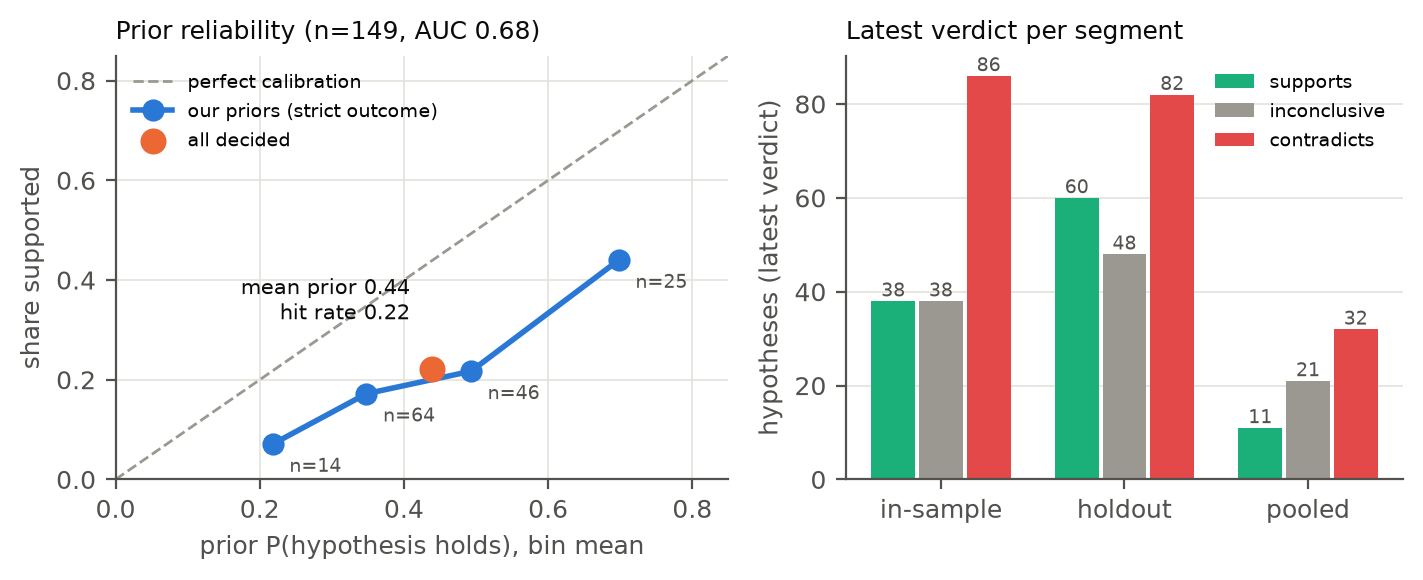
\includegraphics[width=0.88\textwidth]{figures/calibration_now.png}
\caption{Left: reliability of our pre-registered priors (strict outcome: 1 = supported in both segments, 0 = refuted or flipped; open and untested excluded), computed with the rules of \protect\path{scripts/knowledge_book.py} from \protect\path{research/hypotheses.yaml} and \protect\path{research/hypotheses_results.jsonl} as of 2026-11-15. Right: latest verdict per segment over all hypotheses with a result.}
\label{fig:calib}
\end{figure}

%=====================================================================================================
\section{Models}
%=====================================================================================================

Every model below is a deterministic research tool. None is ever trained on, or evaluated with, the LLM's decisions.

\subsection{Volatility}

\paragraph{Per-bar and daily models.} The per-bar sigma is a jump-robust, bias-corrected EWMA (\texttt{vol.robust\_bc}). After a jump the excess variance halves in 2--3 hours, so a plain EWMA over-forecasts post-jump variance by about 27\% (\hyp{H-S4}); the corrected estimator wins by 0.05 QLIKE \citep{patton2011} in both segments (\hyp{H-V1b}; in-sample $t=-8.8$, holdout $t=-3.6$). For daily variance the multi-scale HAR \citep{corsi2009} beats the single-scale EWMA by 0.08 QLIKE in both segments (\hyp{H-VCL1}). The best daily model for crypto is the per-asset log-HAR,
\begin{equation}
\log RV_{t+1} = \beta_0 + \beta_d \log RV_t + \beta_w \overline{\log RV}_{t-6:t} + \beta_m \overline{\log RV}_{t-29:t} + \varepsilon_{t+1},
\end{equation}
mapped back to variance through a Student-$t$ density (log-HAR-$t$). In a 25-model tournament on 23 perps it improved QLIKE on level HAR by 12\% in-sample and 4\% in the holdout, while GARCH-$t$, EGARCH, EWMA and range-based estimators lost (Figure~\ref{fig:vol}, left; \hyp{H-VM2}, \hyp{H-VM5}). Short-history and TradFi perps use a panel HAR pooled across assets. Three refinements did \emph{not} help: range estimators (Garman--Klass HAR is 5\% / 16\% worse), BTC spillover and compression terms, and the sign of the move: crypto has no leverage effect (0 of 23 GJR asymmetry terms significant; \hyp{H-LEV2}).

\paragraph{The calendar.} Weekends are quiet: realised variance over the TradFi weekend window is a median 0.77$\times$ the Friday sigma over 326 weekends (0.82$\times$ in the holdout; \hyp{H-W1}). But weekends are jump-prone, and shrinking the \emph{risk} sigma for them worsened QLIKE in both segments (\hyp{H-V2}, prior 0.75, refuted), so expectations use the weekend-scaled sigma and stops use the unshrunk \texttt{sigma\_risk\_next}. Intraday, an expanding hour-of-week factor $f_h$ applied as $\hat\sigma^2_{t+1} = f_{h(t+1)}\,\hat\sigma^2_{\text{rb},t}$ cuts next-hour QLIKE by 0.040 / 0.076 for crypto and 0.29 / 0.38 for TradFi perps (in-sample / holdout; \hyp{H-NS4}). Variance peaks Sunday 22:00--02:00 UTC and at the US cash open (Figure~\ref{fig:vol}, right). After volatility spikes all forecasts run hot: in the high-volatility regime state, next-week realised variance comes in 13--31\% further below the EWMA forecast than in calm states ($t=-10.9$ in-sample, $-5.0$ holdout, 9 assets; \hyp{H-RL2}).

\paragraph{Machine-learned volatility.} Small MLPs and gradient-boosted trees beat log-HAR for next-day crypto variance in both segments (MLP $-8.0\%$ QLIKE in-sample, $t=-2.9$; XGBoost $-15.7\%$ in the holdout, $t=-2.4$, 22 of 23 symbols; \hyp{H-NN1}), but log-HAR plus weekday dummies already gets $-5.5\%$, and attribution shows the models run on the volatility level (about 40\% of TreeSHAP) and the forecast weekday (Saturday about 0.5--0.6$\times$, Monday about 1.3$\times$) (\hyp{H-NN3}). 95\% of the daily network's weights can be pruned without a detectable loss (\hyp{H-SP1}). For next-hour variance the nonlinear models beat robust sigma $\times$ hour-of-week in both segments (XGBoost $-0.040$ / $-0.065$ QLIKE; \hyp{H-NN8}), about half from extra inputs (recent $|r|$ at 1--24 hours, the daily HAR level) and half from nonlinearity. A frozen hourly model (H-NN10) has been on forward probation since 2026-11-12.

\begin{figure}[t]
\centering
\begin{subfigure}{0.53\textwidth}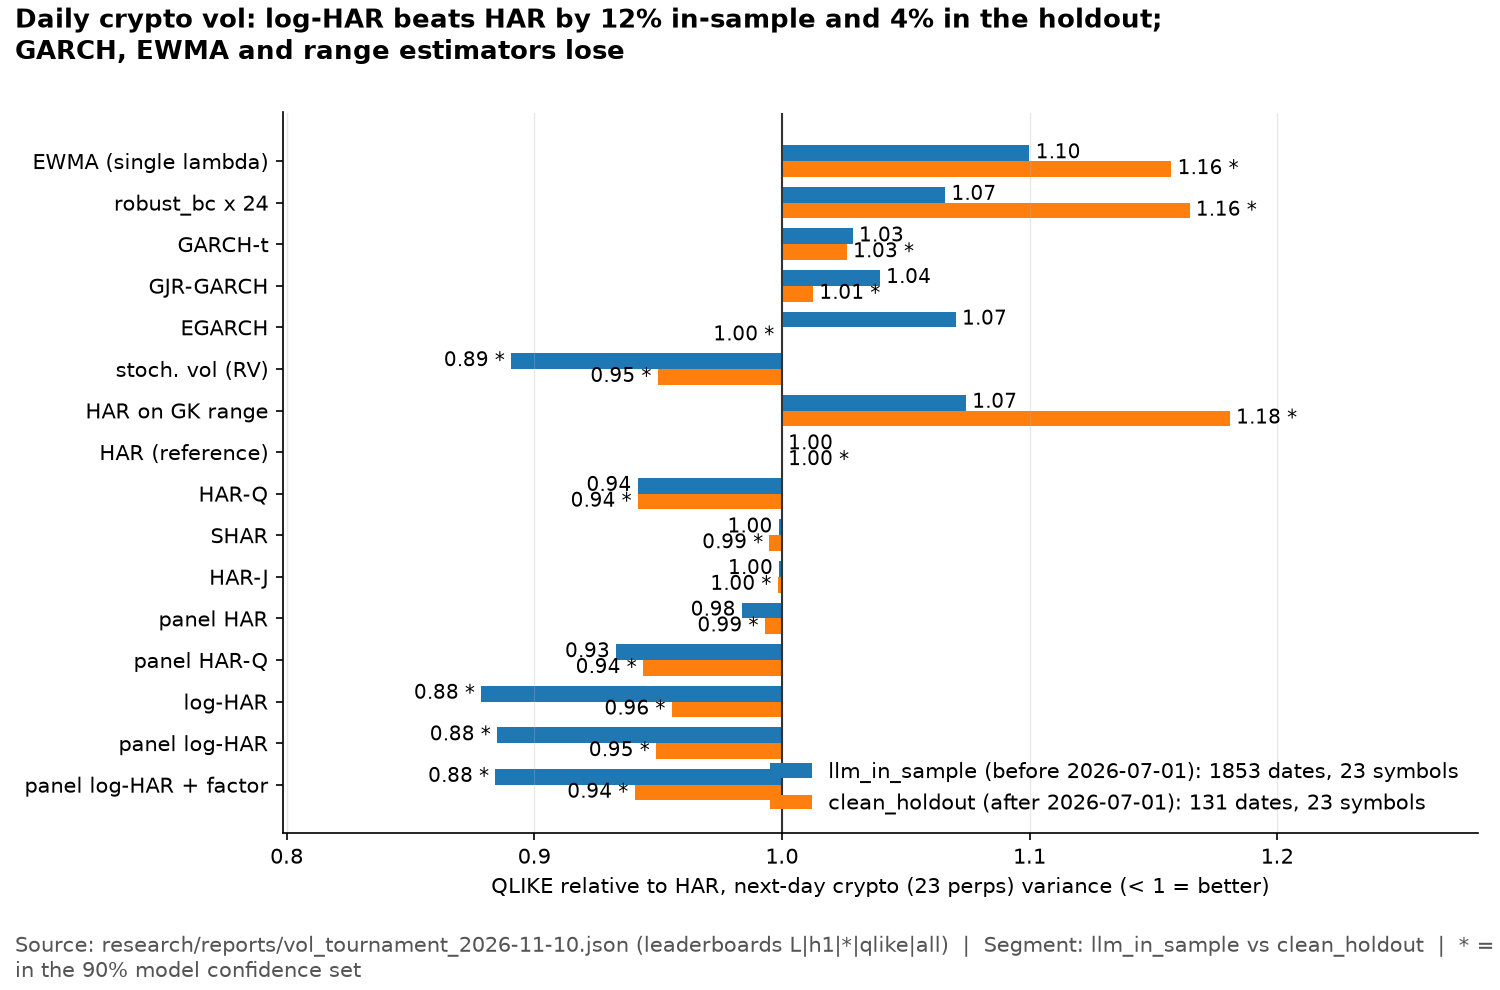
\includegraphics[width=\linewidth]{figures/vol_tournament_crypto_daily.png}\end{subfigure}\hfill
\begin{subfigure}{0.45\textwidth}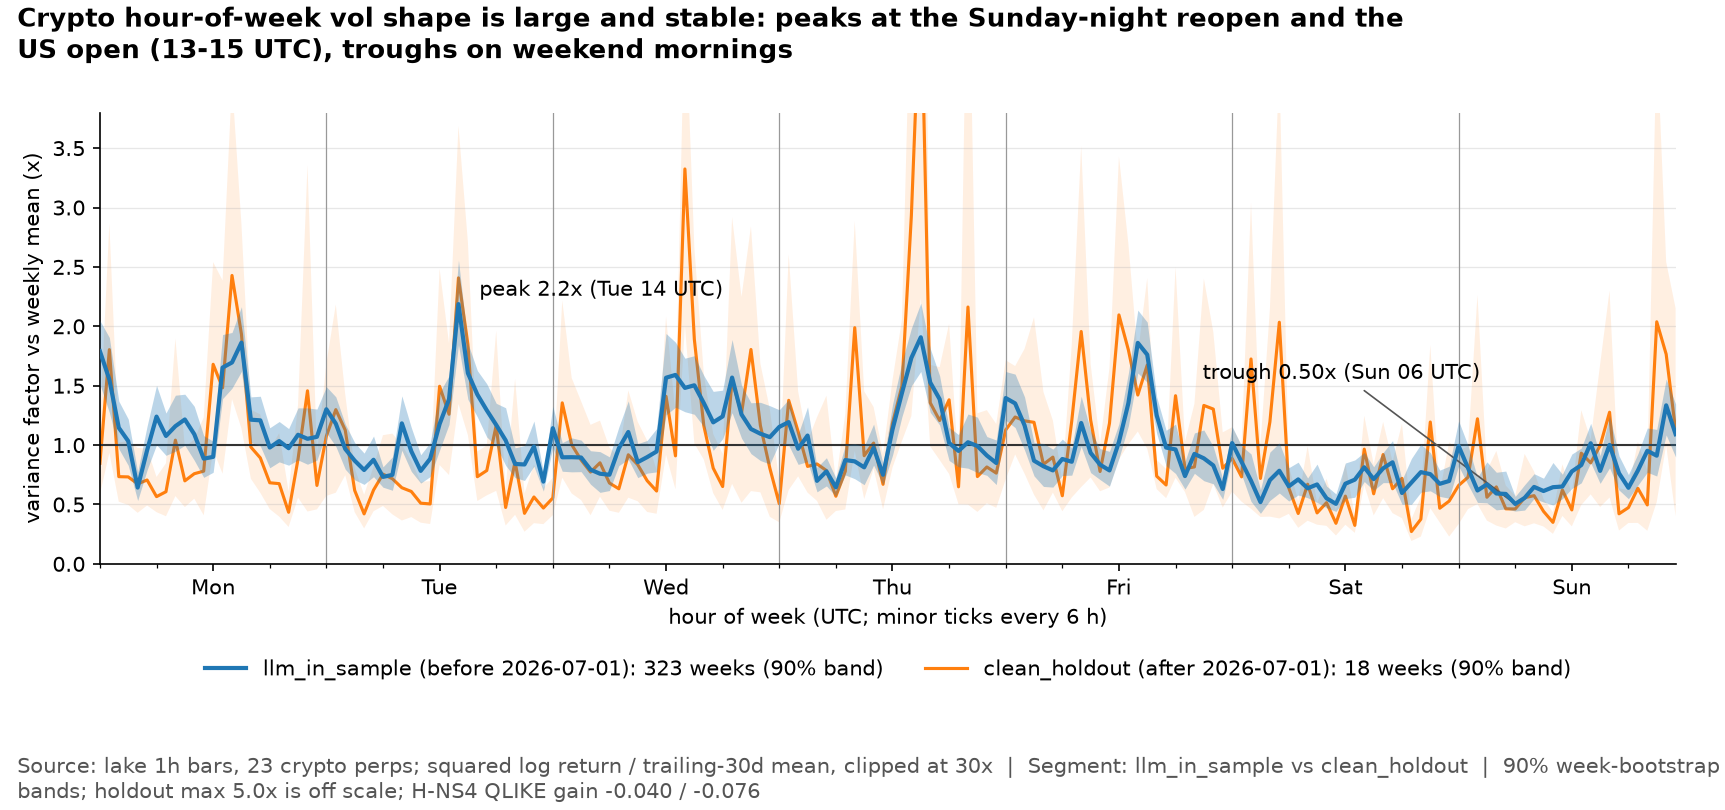
\includegraphics[width=\linewidth]{figures/vol_hour_of_week_crypto.png}\end{subfigure}
\caption{Left: next-day variance tournament on 23 crypto perps, QLIKE relative to level HAR (\protect\path{research/reports/vol_tournament_2026-11-10.json}). Right: the crypto hour-of-week volatility profile (\hyp{H-NS4}), recomputed from lake 1h bars.}
\label{fig:vol}
\end{figure}

\subsection{The probability field}

The BTC probability field (\protect\path{research/reports/btc_field_2026-11-13.md}) asks whether the one-hour return law can be written as a small set of interpretable equations. The hourly log return is modelled as a jump diffusion,
\begin{equation}
r_{t+1} = \mu + \sqrt{D_t}\,\bigl(\epsilon_{t+1} + \mathbb{1}[\text{jump}]\,K_{t+1}\bigr),\qquad \epsilon \sim t_\nu,
\end{equation}
whose drift $\mu/\sqrt{D}$, diffusion $\ln D$ and jump intensity $\ln p_{\text{jump}}$ are sparse polynomials of standardised state coordinates (fast and slow volatility ratios $x_1, x_2$, long-run level $L$, hour-of-week $s = \tfrac12 \ln f$, 24-hour momentum $m_{24}$, trend direction, funding, open interest). Coefficients come from Kramers--Moyal moment regressions on 220 candidate terms with stability selection, refitted monthly from 2022 (59 refits) and frozen at the cutoff on 51k hours. The surviving law is
\begin{align}
\ln D &= \ln v_f - 0.151 - 0.154\,\tilde x_1 - 0.059\,\tilde x_2 + 0.556\,\tilde s - 0.112\,\tilde L\tilde s + 0.145\,\tilde m_{24}\widetilde{\text{dir}},\\
\ln p_{\text{jump}} &= -4.147 + 0.082\,\tilde m_{24}\widetilde{\text{dir}}, \qquad \mu/\sqrt{D} = 0.0142,
\end{align}
with Kou jump sizes, a 1.58\% hourly jump probability and Student-$t$ innovations with 4.3 degrees of freedom. In words: variance follows an amplified hour-of-week profile and a mean-reverting log-volatility (half-life 107 hours, symmetric in the sign of the move), the fast EWMA overshoot is pulled back, the intraday swing is smaller when long-run volatility is high, and variance and jump risk rise when momentum and trend agree (sign-symmetric, so no direction). Only a constant drift survived. A two-dimensional Fokker--Planck solution of the reduced field reproduces the Monte-Carlo quantiles of the 24-hour return.

Against log-HAR-$t$ with constant jumps the field gains $+0.033$ / $+0.051$ nats of log score per origin at 1 hour and $+0.027$ / $+0.062$ at 4 hours (in-sample / holdout, all $t>5$; \hyp{H-FLD1} supported). But against log-HAR-$t$ multiplied by the hour-of-week factor it ties at 1 hour and loses at 4 and 24 hours (Figure~\ref{fig:fieldpnn}, left): the gain is the calendar. The drift carries no direction skill (Brier skill of $P(R>0)$ within $\pm 0.008$, all CIs include 0; \hyp{H-FLD2}), and online recursive updating adds nothing because the coefficients are stable (\hyp{H-FLD3}). The field's main use is the touch-probability card shown on the dashboard.

\subsection{The polynomial-neuron network (KAN-style) and the live networks}

\paragraph{Architecture.} The polynomial-neuron network (PNN, \protect\path{src/ai_trader/ml/pnn.py}) is a Kolmogorov--Arnold-style network \citep{liu2024kan} in which each edge $i\to j$ carries its own univariate function
\begin{equation}
\phi_{ji}(x) = w_{ji}\,\mathrm{silu}(x) + \sum_{d=1}^{4} c_{jid}\,T_d\bigl(\tanh(0.5\,x)\bigr),
\end{equation}
with $T_d$ the Chebyshev polynomials, and each node outputs $b_j + \sum_i \phi_{ji}(x_i)$. The 1-hour model maps 19 standardised inputs (log base variance, the hour-of-week factor, recent absolute returns at 1--24 hours, HAR levels, jump and funding clocks, day-of-week) through a 4-unit latent bottleneck to seven non-crossing quantiles ($\tau \in \{0.05,\dots,0.95\}$; each quantile is the median plus or minus cumulative softplus increments). It has 531 parameters; an equal-size ReLU MLP (519 parameters) is the control.

\paragraph{Training and validation.} Both families are trained identically with AdamW on the pinball loss averaged over the seven quantiles, with early stopping on a validation block, in a walk-forward of 65 monthly refits (2021-07 to 2026-11) at 1 hour and 64 at 1 day, two seeds each, under a 2,000-parameter cap. Intervals are conformalised with CQR scores \citep{romano2019} and adaptive conformal inference \citep{gibbs2021}, $\alpha_{t+1} = \alpha_t + \gamma(\alpha - \text{err}_t)$ with $\gamma = 0.005$ and a 1,440-hour window.

\paragraph{Results.} At 1 hour the network beats log-HAR-$t$ in both segments (pinball $-0.00082$, $t=-7.3$ in-sample; $-0.00124$, $t=-3.0$ holdout), but so does the equal-size MLP, and the polynomial edges add nothing over ReLU ($+0.00002$, $t=0.2$; $-0.00027$, $t=-1.1$). At 1 day nothing beats log-HAR-$t$ (Figure~\ref{fig:fieldpnn}, right; \hyp{H-PNN1} refuted). ACI holds 1-hour holdout coverage within 0.2 percentage points of nominal, but its bands are 2--3\% wider than log-HAR-$t$'s, which is already within about 2 points of nominal (\hyp{H-PNN2} open). The 4-unit latent state is predictable (holdout $R^2$ gain over persistence 0.14 at 1 hour), but feeding its prediction back changes nothing (\hyp{H-PNN3} open). Symbolic extraction recovers known structure: about a third of the 1-hour encoder edges are cubics with $R^2\ge 0.99$, and the dominant inputs are the hour-of-week factor and the last hour's $|r|$.

\begin{figure}[t]
\centering
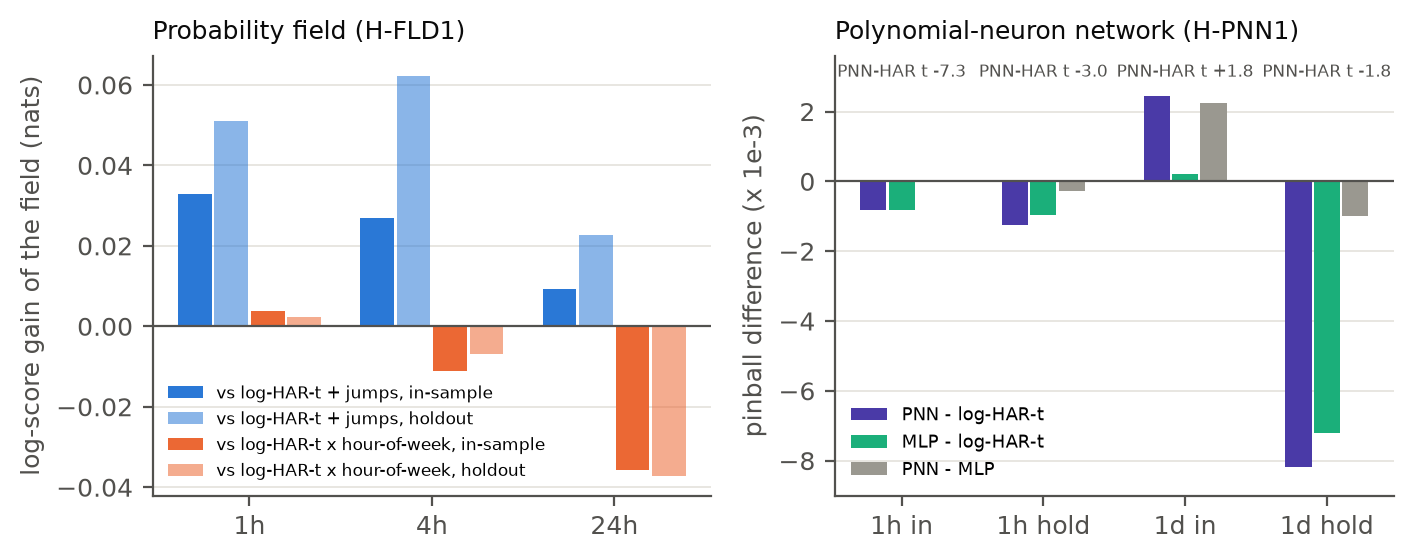
\includegraphics[width=0.97\textwidth]{figures/field_pnn_scores.png}
\caption{Left: log-score gain of the probability field over log-HAR-$t$ with constant jumps (blue) and over log-HAR-$t$ $\times$ hour-of-week (orange), from \protect\path{research/reports/btc_field_2026-11-13.md}. Right: pinball-loss differences of the PNN and the equal-size MLP against log-HAR-$t$, and PNN minus MLP (negative is better), from \protect\path{research/reports/btc_pnn_2026-11-13.md}.}
\label{fig:fieldpnn}
\end{figure}

\paragraph{Live v1 and v2.1.} Despite the null on polynomial structure, the frozen 1-hour and 1-day PNNs (refit 2026-11, two seeds averaged) became the live hourly line \texttt{live\_nn.v1} (\protect\path{src/ai_trader/live/nn.py}), because they are calibrated, cheap and interpretable. Each run at hh:03 UTC reads the lake as of that time, forecasts the next hour and a rolling 24 hours, applies ACI at 80/90/95\%, adds the field card, the latent state, the H-NN10 volatility line and news attention features, scores every forecast whose window has closed, and raises alarms when running coverage leaves its binomial 99\% interval. Version \texttt{v2.1} (\protect\path{src/ai_trader/live/nn_v2.py}) is a shadow that differs only in the conformal layer: $\gamma = 0.02$, bands issued at $\max(\alpha_t, \alpha/4)$ so they never become infinite, and a floor during jump clusters at the largest of the network, field and H-NN10 sigmas. It was declared in the diary before any live v2 line existed. The neuron atlas (\protect\path{research/reports/brain_atlas_2026-11-15.md}) dissects the frozen 1-hour network: the hour-of-week factor is the top input of all eight latent units, the latent core is first of all a weekly clock, the two seeds learn mirror-image units, and the whole network beats a constant forecast by only about 4\% of pinball (Figure~\ref{fig:brain}).

\begin{figure}[t]
\centering
\begin{subfigure}{0.49\textwidth}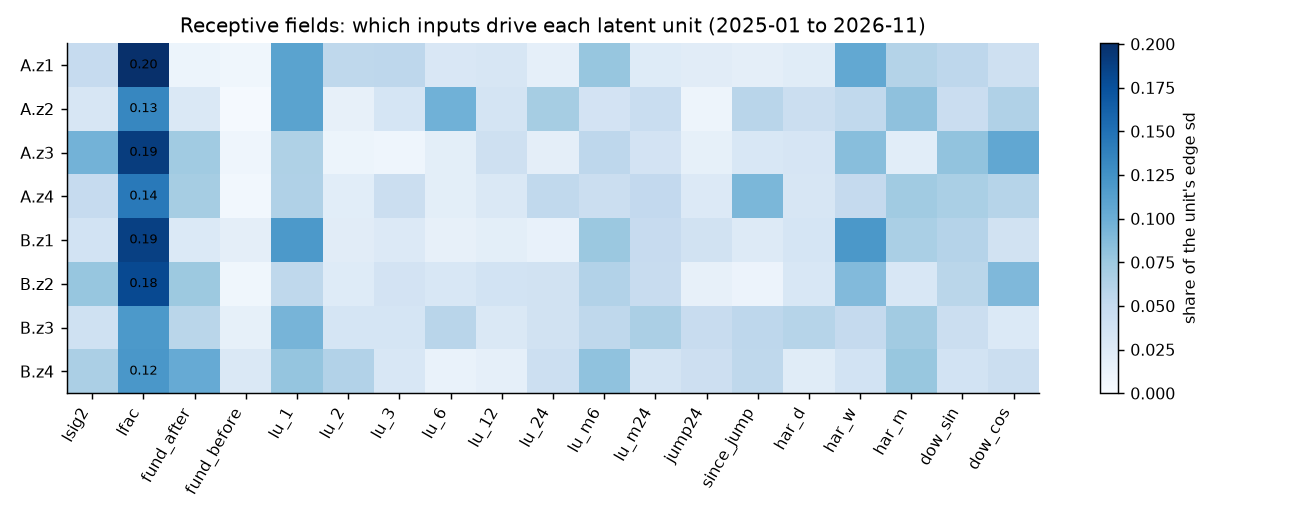
\includegraphics[width=\linewidth]{figures/brain_receptive_fields.png}\end{subfigure}\hfill
\begin{subfigure}{0.49\textwidth}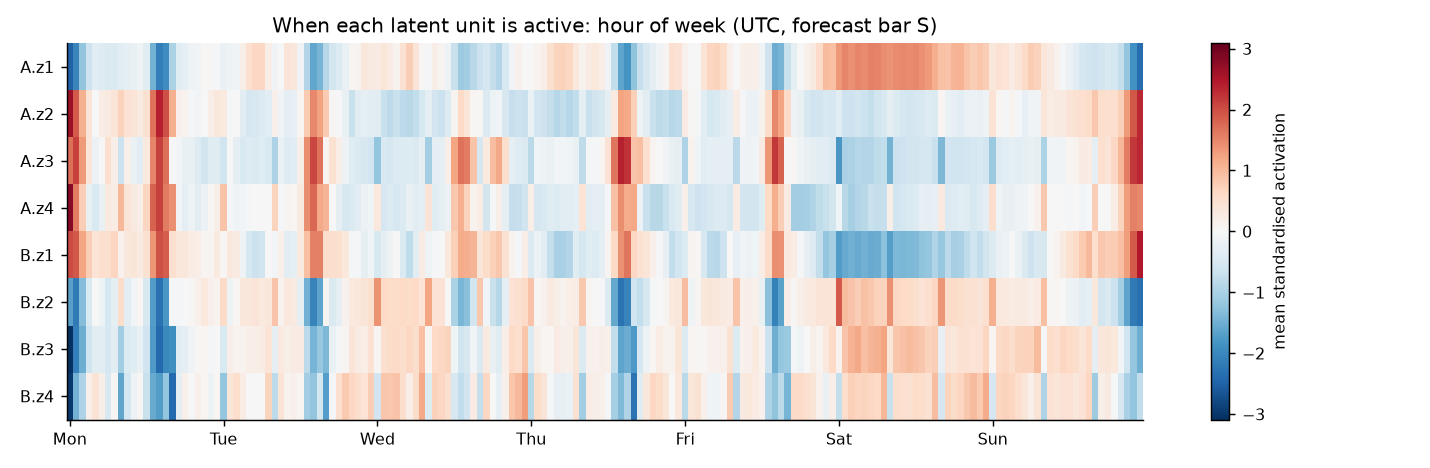
\includegraphics[width=\linewidth]{figures/brain_hour_of_week.png}\end{subfigure}
\caption{Neuron atlas of the frozen live 1-hour PNN (\protect\path{research/reports/brain_atlas_2026-11-15.md}; descriptive, not a test). Left: receptive fields, the share of each latent unit's edge variation by input. Right: mean activation of each latent unit by hour of week.}
\label{fig:brain}
\end{figure}

\subsection{The cross-sectional network v3}

The cross-sectional network (\protect\path{research/reports/xs_network_2026-11-15.md}) applies a shared polynomial-edge encoder to each of the 23 universe-L tokens, mixes tokens with an attention layer, and outputs 1- and 4-hour volatility quantiles and 4- and 24-hour quantiles of each token's return relative to the equal-weight basket. It has 4,147 parameters (an MLP arm has 4,127), was refitted 18 times quarterly from 2022Q3 with purging, three seeds per arm. The volatility head beats panel log-HAR-$t$ $\times$ hour-of-week at 1 hour by 1.4\% of pinball in both segments, for every one of the 23 tokens (\hyp{H-XS2} supported). The relative-return head ranks tokens with a rank IC of 0.052 at 4 hours and 0.061 at 24 hours in the holdout, beating momentum and reversal (\hyp{H-XS1} supported), but a free ranking by low current volatility already reaches 0.039 / 0.060, the network adds only $+0.013$ at 4 hours over it, and the top-minus-bottom quintile spread is $-12$ / $-29$\,bp after costs in the holdout. Attention across tokens helps in-sample and hurts in the holdout (\hyp{H-XS3} flips); BTC and TRX, the low-volatility anchors, are the attention hubs. Polynomial edges again add nothing over the MLP arm. v3 runs live as context only (\protect\path{src/ai_trader/live/xs_v3.py}); the decision sessions do not read it.

\begin{figure}[t]
\centering
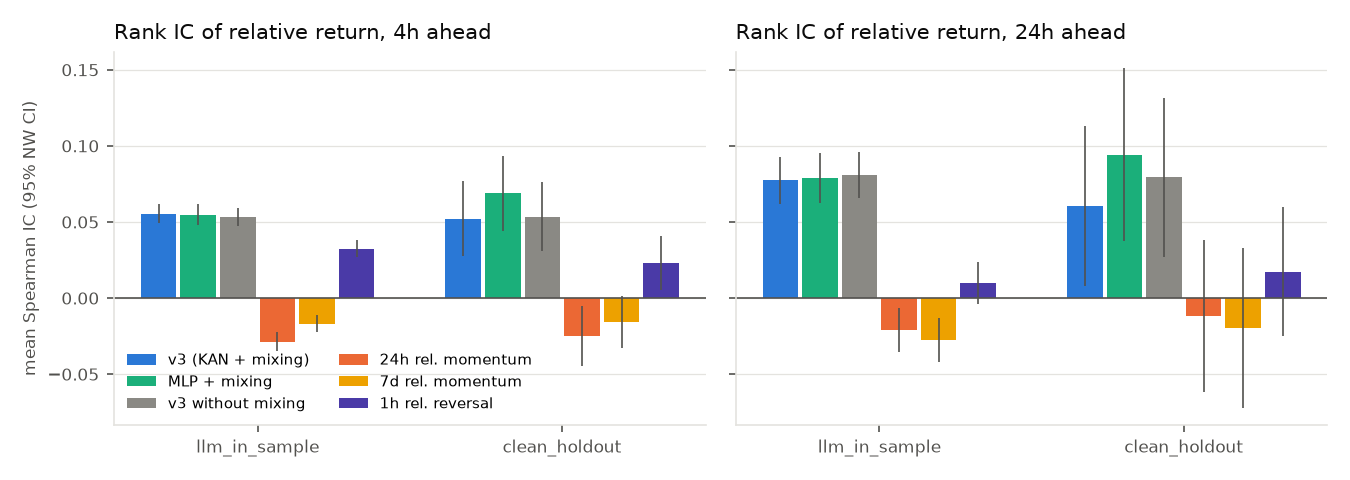
\includegraphics[width=0.92\textwidth]{figures/xs_ic_vs_baselines.png}
\caption{Rank IC of predicted relative returns for v3, the MLP arm, v3 without mixing and three simple baselines (\protect\path{research/reports/xs_network_2026-11-15.md}). The IC is genuine median-forecasting skill but mostly a low-volatility ranking, and it does not survive costs as a long-short spread.}
\label{fig:xs}
\end{figure}

\subsection{The order-book generator and the matching engine}

To simulate execution at the order level the project wrote \texttt{at-match} (\protect\path{crates/at-match}, \protect\path{docs/MATCHING_ENGINE.md}), a deterministic limit order book with Bybit v5 semantics: price-time priority, partial fills that keep queue position, amendments that lose priority, GTC/IOC/FOK/PostOnly time-in-force, reduce-only, instrument filters and maker/taker fees, with trade and \texttt{orderbook.200}-shaped outputs. It has no internal clock, and it replays a real ob200 day exactly. It deliberately does not model what Bybit does not publish (liquidation engine, ADL, mark price, internal latency). A queue-reactive order-flow generator calibrated on three ob200 days and run through the engine reproduces 6 of 8 held-out book and trade facts on 31 days (spread state, depth, queue depletion, size, inter-arrival, impact, $|r|$ autocorrelation), but signed-flow autocorrelation is too weak (0.003 against 0.011) and taker sizes too small (\hyp{H-OBG1} supported). Generated twin days did not help a next-minute volatility model and hurt when real data were cut to 25\% (QLIKE ratio 1.006, CI above 1; \hyp{H-OBG2} refuted). The engine's main use turned out to be replaying our own quoting code on real books (Section~\ref{sec:results}).

\subsection{The vector-open level framework (vecopen)}

\texttt{vecopen} is a separate, specification-driven build (\protect\path{vecopen/SPEC.md}) of an idea brought by the operator: that the open of the candle that starts a displacement leg (2.0 ATR) is a level price returns to. It splits the idea into two falsifiable claims: \hyp{H-VO1}, the first return to an untouched leg-origin open resolves (leaves a $\pm k$ ATR band) more often and further than at matched placebo levels; and \hyp{H-VO2}, such levels are magnets, touched more often than placebo levels at the same distance and more than a driftless diffusion predicts. The build runs in gated phases with a hash-chained, tamper-evident trial registry. Phase 0 (scaffold), phase 1 (Binance 5-minute data for 20 crypto assets, holdout locked and unreadable), phase 2 (streaming level registry, 12 hand-built cases) and phase 3 (events, triple-barrier labels and three placebo families, 349,259 matched pairs) are complete. Phase 3 failed one balance criterion on monthly levels (standardised mean difference 0.177 on 31 pairs); the build stopped, and the operator chose to judge balance by timeframe group, using covariates only and changing no parameter. Gate G1, a leak audit by a fresh-context auditor (truncation, perturbation and timestamp tests), passed on all 20 assets. Gate G2, the treated-versus-placebo event study, has not been run: it waits for 10+ years of CFD data (FX, indices, metals, energy, bonds) from a cTrader account, which the monthly and weekly levels need. No outcome statistic comparing treated and placebo levels has been computed.

%=====================================================================================================
\section{Results across the research programmes}
\label{sec:results}
%=====================================================================================================

The work ran as numbered programmes, each with hypotheses registered before the agents started: weekends and the foundations (2026-11-07/08), volatility (27 hypotheses, 2026-11-10), strategies (22 hypotheses, 2026-11-10/11), microstructure (one-day pilot, then 31 random days), an overnight ML programme (2026-11-12), the BTC field programme (field, PNN, news, order-book generator; 2026-11-13), and side studies on 2026-11-14/15 (market-making replay, options, execution, post-crash, cross-section). Figure~\ref{fig:verdicts} summarises the status of all 252 hypotheses by group, and Table~\ref{tab:results} lists the main ones.

\begin{figure}[t]
\centering
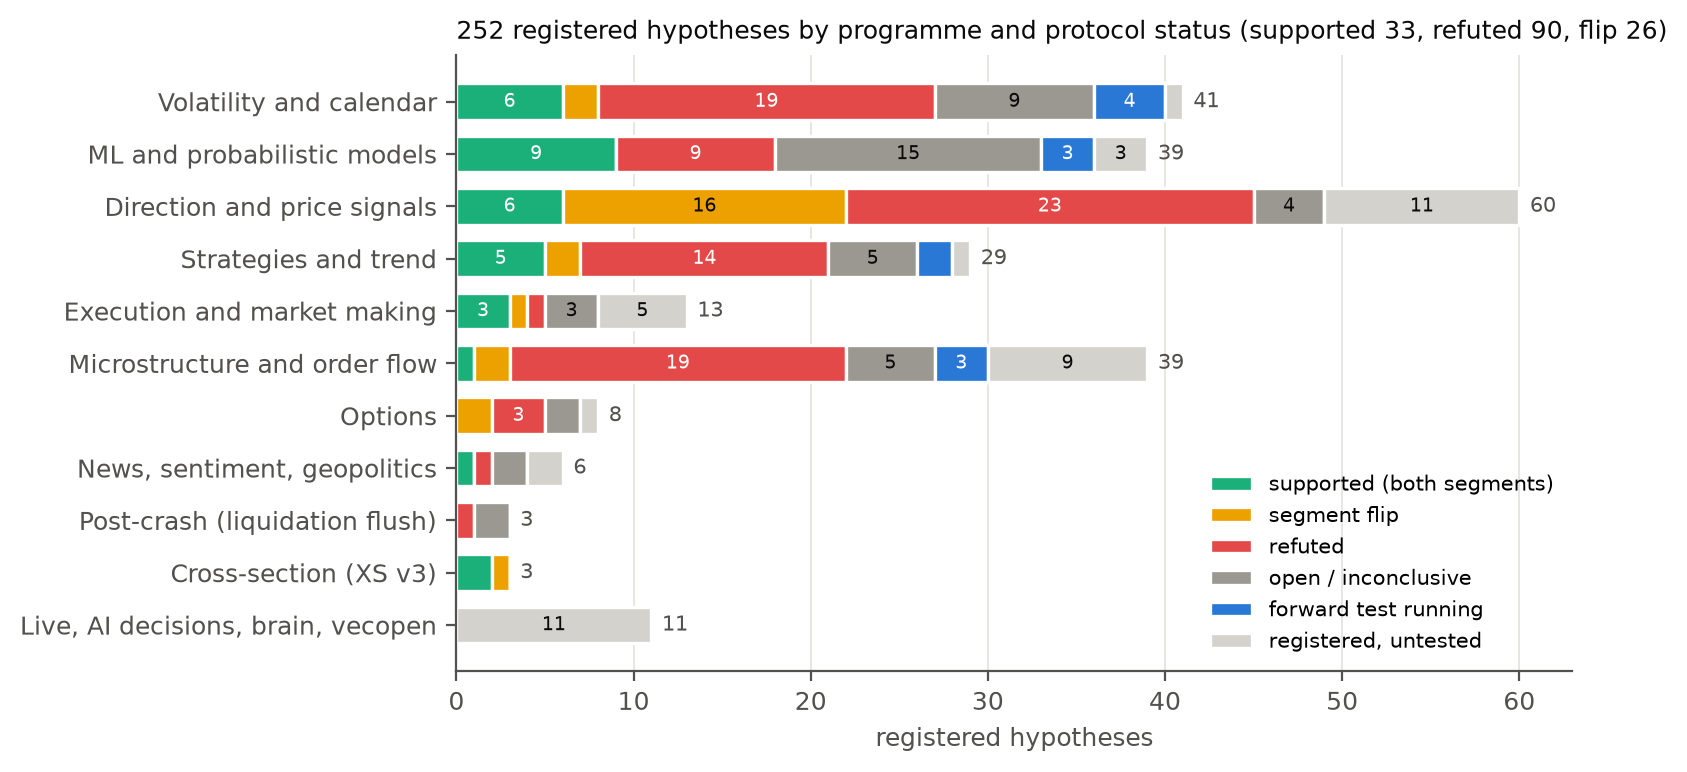
\includegraphics[width=0.88\textwidth]{figures/verdicts_by_group.png}
\caption{Protocol status of the 252 registered hypotheses, grouped by programme (families mapped to groups in \protect\path{paper/make_figures.py}). ``Supported'' needs support in-sample and the same sign in the holdout; a segment flip counts as not supported.}
\label{fig:verdicts}
\end{figure}

{\small
\begin{longtable}{@{}>{\raggedright\arraybackslash}p{1.55cm}>{\raggedright\arraybackslash}p{6.1cm}cc>{\raggedright\arraybackslash}p{5.3cm}@{}}
\caption{Main hypotheses: latest verdict in \seg{llm\_in\_sample} / \seg{clean\_holdout} (S supports, X contradicts, ? inconclusive, -- not run) and the key number. Sources: \protect\path{research/hypotheses_results.jsonl}, \protect\path{research/BELIEFS.md} and the reports named in the text.}\label{tab:results}\\
\toprule
ID & Hypothesis & In & Hold & Key number \\
\midrule
\endfirsthead
\toprule
ID & Hypothesis & In & Hold & Key number \\
\midrule
\endhead
\multicolumn{5}{@{}l}{\emph{Volatility and calendar}}\\
H-W1 & Weekends are quiet & S & S & RV 0.77$\times$ Friday $\hat\sigma$ (0.82 holdout) \\
H-V2 & Shrink the risk sigma over weekends & X & X & weekends are jump-prone; prior was 0.75 \\
H-S4, V1b & Post-jump vol decays; bias-corrected robust EWMA & S & S & half-life 2--3\,h; QLIKE $-0.05$ \\
H-VCL1 & Multi-scale HAR beats EWMA & S & S & QLIKE $-0.079$ / $-0.087$ \\
H-NS4 & Hour-of-week profile & S & S & crypto QLIKE $-0.040$ / $-0.076$ \\
H-RL2 & High-vol states over-forecast next week & S & S & 13--31\% below EWMA; $t$ $-10.9$ / $-5.0$ \\
H-LEV2 & No leverage effect in crypto & S & S & 0/23 GJR terms significant \\
H-W7 & Implied vol overprices the weekend & S & S & BTC RV/IV 0.35 vs 0.84 weekdays ($t$ $-17$) \\
H-OPT1 & Selling the Friday weekend straddle pays & X & X & premium real, trade loses net \\
\multicolumn{5}{@{}l}{\emph{ML and probabilistic models}}\\
H-NN1 & Nonlinear daily vol beats log-HAR & S & S & XGB $-15.7\%$ holdout; mostly weekday \\
H-NN8 & Nonlinear next-hour vol & S & S & XGB QLIKE $-0.040$ / $-0.065$ \\
H-FLD1 & Probability field beats log-HAR-$t$ & S & S & $+0.051$ nats at 1\,h (holdout); calendar only \\
H-PNN1 & Polynomial neurons beat MLP / HAR & X & ? & PNN $=$ MLP; nothing beats HAR at 1\,d \\
H-XS2 & Cross-sectional 1\,h vol beats panel HAR & S & S & pinball $-1.4\%$, all 23 tokens \\
H-XS3 & Cross-token attention adds information & S & X & holdout pinball lower without it \\
H-OBG2 & Generated books help train vol models & X & X & QLIKE ratio 1.006 at 25\% real data \\
\multicolumn{5}{@{}l}{\emph{Direction and price signals}}\\
H-S2 & Shocks into calm markets continue, into volatile ones reverse & -- & S & forward-supported once; grade B/C \\
H-T1 & Hourly 2$\sigma$ deviations continue & -- & S & fading loses before costs \\
H-NN2, NN6 & ML has no direction skill (null) & S & ?/S & Brier skill $\approx 0$; next-minute AUC 0.505 \\
H-RL1 & Regime cells predict next-week return & X & S & up$-$down 0.03$\sigma$, $t$ 1.0 \\
H-VZ1 & Vector-open levels hold on first touch & X & X & break rate 0.52--0.55 \\
H-AU1 & Market-profile acceptance continues & X & S & flip: not supported \\
H-P1 & Funding contrarian & X & S & flip: not supported \\
H-C1 & Funding carry is harvestable & S & S & net Sharpe 2.8 in-sample; decayed to $-4.8\%$/yr in 2026H1 \\
\multicolumn{5}{@{}l}{\emph{Strategies and trend}}\\
H-TR1 & Equal-weight trend ensemble earns & S & X & $+0.33$ Sharpe in-sample, negative holdout \\
H-TR2 & Walk-forward selection beats the ensemble & X & X & winner's DSR 0.72 $<$ 0.95 \\
H-PD1 & The book is several independent bets & X & X & 1.15 effective bets (2.5 holdout) \\
H-PD4 & Gross-to-net gap is exits, not fees & S & S & exits+costs 70--75\% of favourable excursion \\
H-VBOS3 & Vol break of structure improves trend & X & X & DSR 0.22, PBO 0.84 \\
H-TP1 & Stock perps revert at the US open & ? & X & fading overnight moves $-67$\,bp net \\
\multicolumn{5}{@{}l}{\emph{Execution and market making}}\\
H-EXE1 & Limit at the touch beats market entry & S & S & $+0.010$\,R/signal; 275/275 filled \\
H-MMR0 & Replay reproduces live MM fills & -- & S & 6/6 P\&L signs (7 live fills) \\
H-MMR1 & Passive quoting nets $>0$ on held-out days & -- & ? & BTC $+0.039$\,USD/day, CI $[-0.11, +0.18]$ \\
H-MMR3 & Quoting only in quiet phases turns MM positive & -- & ? & gate removes 99\% of fills; no edge \\
H-JD4 & Jump-aware first-passage odds for brackets & S & S & Brier $-0.0022$ / $-0.0014$ \\
\multicolumn{5}{@{}l}{\emph{Microstructure and order flow}}\\
H-MS1 & Arrivals are not exponential & -- & X & 3-speed mixture fits, but criterion failed \\
H-MD1 & Micro traits are stable per symbol & X & X & ICC 0.23--0.34: calibrate per day \\
H-OF1 & Flow anomalies flag volatility & -- & X & $|z|>4$ fires on 22\% of minutes \\
H-MINE1 & Mined micro effects replicate & \multicolumn{2}{c}{pooled S} & 454/550; vol 90\%, direction 28\% \\
\multicolumn{5}{@{}l}{\emph{Options}}\\
H-OPX1 & Long vol pays after a compression & ? & ? & straddle $-3.9\%$ vs $-6.4\%$ of premium \\
H-OPX2 & Short deep-ITM put beats a same-delta perp & X & ? & $-0.33\%$ of spot per 14 days \\
H-OPX4 & Scale out after an extreme profit & X & X & $-0.0036$\,R/trade (68,641 trades) \\
\multicolumn{5}{@{}l}{\emph{News and sentiment}}\\
H-NEWS3 & News attention improves next-day vol & X & X & QLIKE $+3$--$4\%$ worse \\
H-NEWS4 & News has no direction skill (null) & S & S & Brier skill $-0.018$ \\
\multicolumn{5}{@{}l}{\emph{Post-crash}}\\
H-RB1 & Buy the long-liquidation flush & X & X & $-0.19$\,R / $-0.34$\,R per trade \\
H-RB2 & Short the failed rebound & ? & ? & $-0.00$\,R / $+0.42$\,R (19 trades) \\
\multicolumn{5}{@{}l}{\emph{Cross-section}}\\
H-XS1 & v3 ranks tokens better than momentum/reversal & S & S & holdout IC 0.052 (4\,h); mostly low-vol \\
\multicolumn{5}{@{}l}{\emph{Live, AI and brain (forward only)}}\\
H-AI1 & Claude's take/skip beats RULE and RANDOM & -- & -- & needs $\ge$ 60 closed AI trades \\
H-LIVE1 & Claude's forecasts beat the network & -- & -- & 60 forecasts logged, 1 scored pair \\
H-LT1 & The live desk has positive expectancy & -- & -- & needs $\ge$ 100 closed live trades \\
H-BR1 & Intra-hour nowcast beats frozen bands & -- & -- & recorder running \\
\bottomrule
\end{longtable}
}

\paragraph{Volatility and the calendar.} This is the only area with large, stable effects in both segments, and it is where most grade-A rules come from: weekends are quiet but jump-prone, the hour-of-week shape is large, jumps decay in hours, high-volatility states over-forecast, there is no leverage effect, and a daily forecast is the volatility level plus the weekday. The forecasting gain from machine learning is real but mostly calendar.

\paragraph{Direction.} Every direction test is at coin-flip level. Next-day direction from standard features has Brier skill near zero and gets worse with more inputs (\hyp{H-IC1}); levels (vector-candle opens, pivots, CME gaps, value areas) break slightly more often than they hold; Monday drift, regime direction, funding contrarian, OI divergence, stablecoin growth, variance risk premium, Market Cipher dots and Kalman trendiness all fail. Of 60 direction and price-signal hypotheses, 6 are supported, and those are mostly nulls (``no skill'') or the shock and trend continuation patterns, graded B or C.

\paragraph{Strategies and trend.} The 16-sleeve deterministic book is about one crypto trend bet (1.15 effective bets in-sample) with a thin edge before the cutoff and a negative one after it. Per-symbol parameter selection is a coin flip (PBO 0.44 for the trend zoo, 0.65 for breakouts; \hyp{H-SYN1}); per-cell strategy rankings do not persist across the cutoff (Spearman 0.085). Regimes say where strategies lose and how long a state lasts, not who wins. Edge leaks through exits rather than fees, and tight trailing exits make it worse because trend profits come from rare large days (\hyp{H-PD6}).

\begin{figure}[t]
\centering
\begin{subfigure}{0.49\textwidth}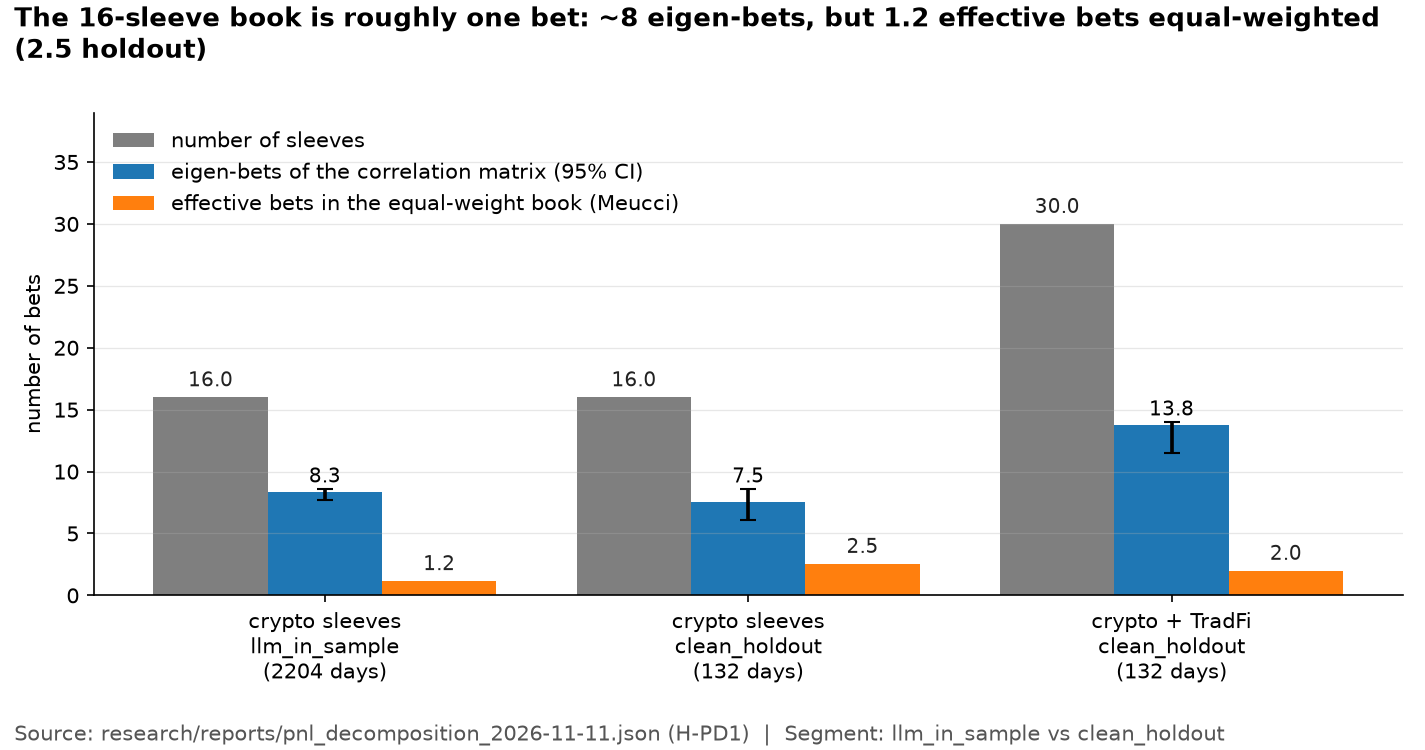
\includegraphics[width=\linewidth]{figures/pnl_effective_bets.png}\end{subfigure}\hfill
\begin{subfigure}{0.49\textwidth}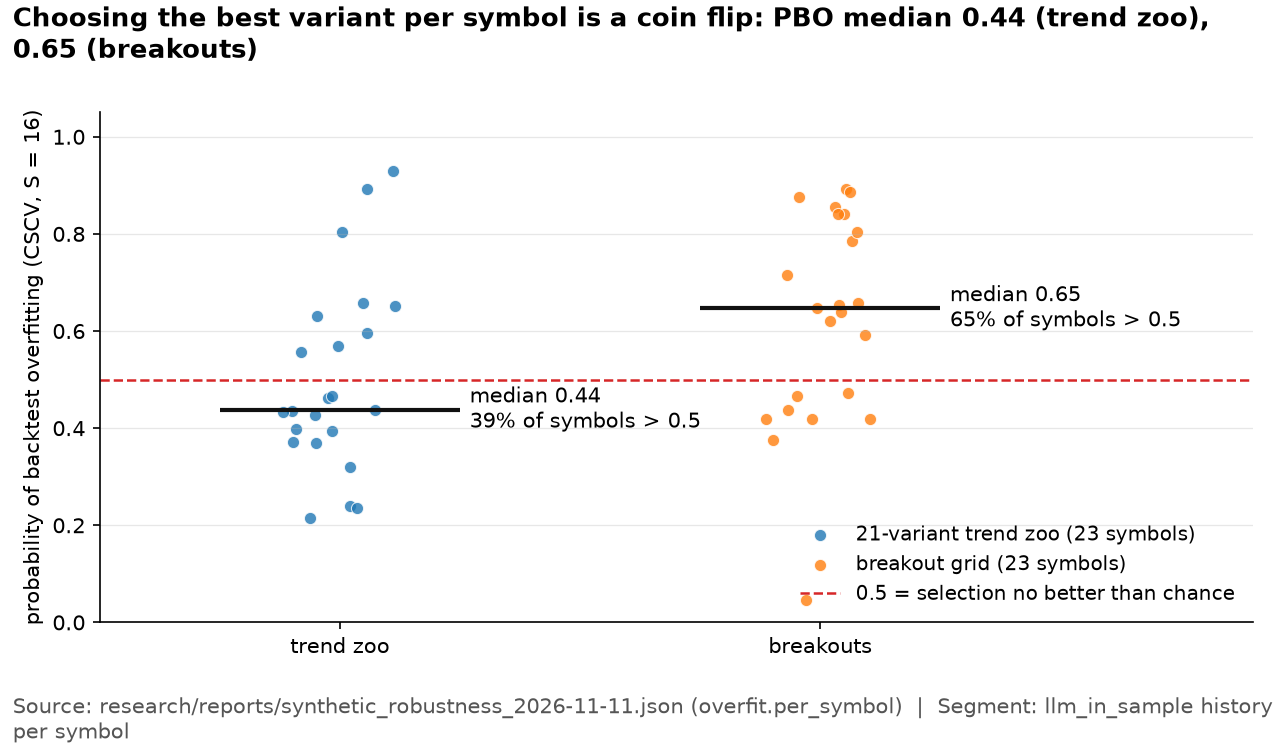
\includegraphics[width=\linewidth]{figures/selection_overfit_pbo.png}\end{subfigure}
\caption{Left: the 16-sleeve book is roughly one bet (\protect\path{research/reports/pnl_decomposition_2026-11-11.md}). Right: choosing the best variant per symbol is a coin flip, with PBO 0.44 (trend zoo) and 0.65 (breakouts) (\protect\path{research/reports/synthetic_robustness_2026-11-11.md}).}
\label{fig:book}
\end{figure}

\paragraph{Execution and market making.} The live market-making runs (2026-11-08 to 2026-11-12) were small: the first hour of the multi-asset quoter closed $+0.04$\,USD on about 994\,USD of turnover, passive exits made money (87\% winners) and market-order exits gave most of it back. Replaying the live quoting code on real Bybit ob200 books (\texttt{atx mm-replay}, 80 symbol-days, all after the cutoff) showed why: quotes within about 25\,bp of mid lose because adverse selection within one second exceeds the spread captured, before fees (Figure~\ref{fig:exec}, left); wide quotes (40--50\,bp) break even at best (\hyp{H-MMR1} inconclusive). Gating quotes to quiet sideways phases reduces adverse selection but not below the 2\,bp maker fee (\hyp{H-MMR3}). The one positive execution result is for the paper sleeves: entering with a PostOnly limit pegged to the touch beat a market order by $+0.010$\,R per signal (CI $+0.009$ to $+0.012$; holdout $+0.014$), all 275 signals filled within 37 seconds, and the gain is the maker-taker fee gap ($+0.015$\,R) minus a slightly worse price ($-0.005$\,R) (\hyp{H-EXE1}).

\begin{figure}[t]
\centering
\begin{subfigure}{0.56\textwidth}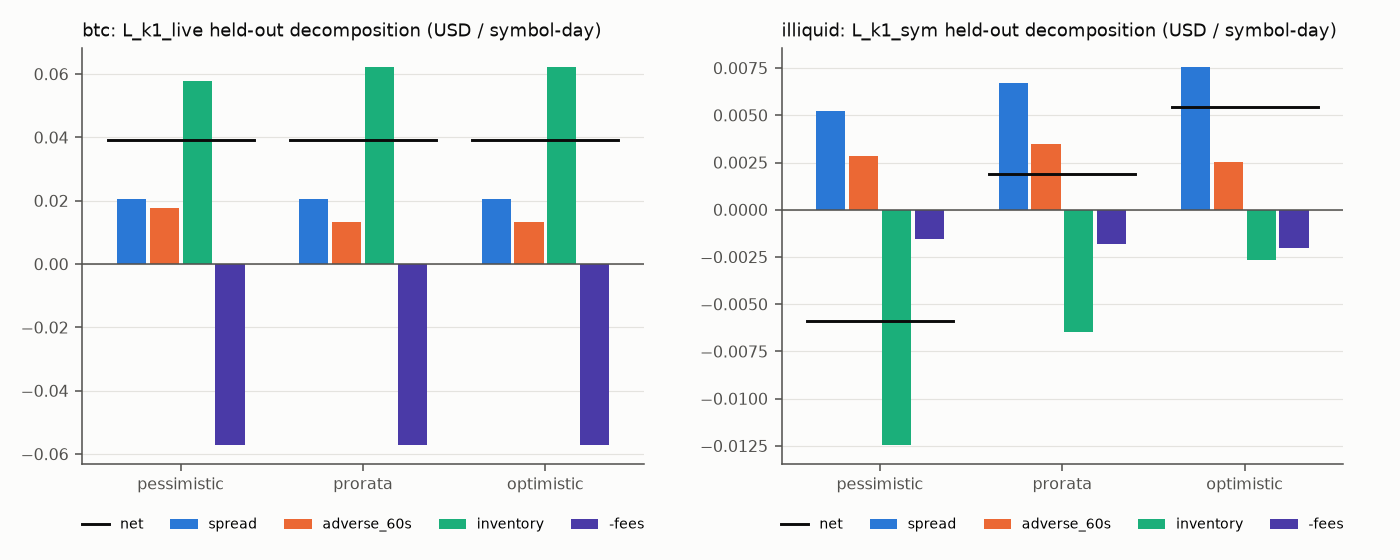
\includegraphics[width=\linewidth]{figures/mm_replay_decomposition.png}\end{subfigure}\hfill
\begin{subfigure}{0.42\textwidth}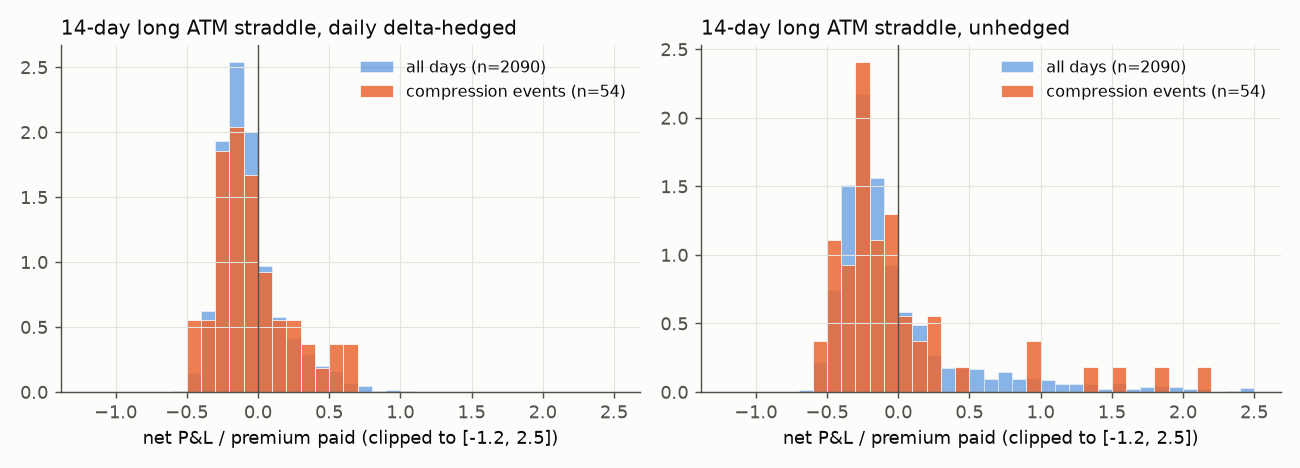
\includegraphics[width=\linewidth]{figures/opx1_straddle.png}\end{subfigure}
\caption{Left: held-out P\&L decomposition of the selected wide quoters on replayed real books, by queue model (\protect\path{research/reports/mm_replay_2026-11-14.md}); fees eat the spread. Right: 14-day long ATM BTC straddles after volatility compressions versus all days (\protect\path{research/reports/options_compression_2026-11-14.md}); options are cheaper after compressions, not mispriced.}
\label{fig:exec}
\end{figure}

\paragraph{Microstructure.} Trade arrivals are bursty (a three-speed exponential mixture), order signs have long memory (power-law ACF, Hurst of signed flow 0.53), sizes have heavy tails, and activity scales across perps roughly as microstructure invariance predicts \citep{kyle2016}. But per-symbol traits vary as much from day to day as across symbols (ICC 0.23--0.34), so simulators must be calibrated per day, and simulated paths cannot rank market-making settings (Spearman $-0.09$ to $0.30$ against real replay). Flow anomalies are an activity gauge, not a direction signal.

\paragraph{Options.} On 24.2 million Deribit BTC option trades (2020--2026), selling weekend volatility from Friday morning lost net in both segments even though implied volatility does overprice weekends. After volatility compressions, long straddles lose less than on other days but still lose (Figure~\ref{fig:exec}, right). A structure the operator proposed, a long call plus a short deep-ITM put, cuts vega by about 74\% but is essentially a 1.1-delta long future with crash exposure, and lost against a same-delta perp at compression events.

\paragraph{News and sentiment.} GDELT could not be used (rate limits; see Section~\ref{sec:lessons}). Wikipedia pageviews and edits, Hacker News counts, the Fear and Greed index, the event calendar and on-chain activity made next-day BTC variance forecasts 3--4\% worse than log-HAR $\times$ weekday, and carried no direction skill.

\paragraph{Post-crash.} After a long-liquidation flush (649 events on 23 perps, 2020--2026), buying the next 4-hour close loses ($-0.19$\,R in-sample, $-0.34$\,R holdout, worse than random longs in the same regime cell): price usually makes a further low a median 8.7\% below the event close, a median 54 hours later, then rebounds about 15\% (Figure~\ref{fig:postflush}). Shorting the first failed rebound is about breakeven.

\begin{figure}[t]
\centering
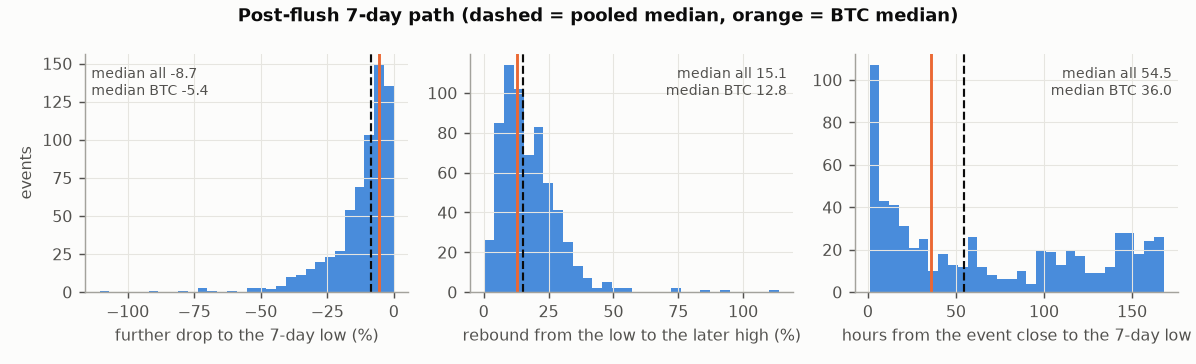
\includegraphics[width=0.95\textwidth]{figures/post_flush_path.png}
\caption{The seven days after a long-liquidation flush (\protect\path{research/reports/post_cascade_2026-11-15.md}): the low is usually still ahead, and comes late; a stop under the flush low is usually hit before the rebound.}
\label{fig:postflush}
\end{figure}

\paragraph{Cross-section and the brain.} The cross-sectional network's ranking skill is real for medians and useless as a long-short spread after costs. The neuron atlas shows that the live network spends much of its capacity re-encoding a deterministic seasonal profile. Both are consistent with the overall reading of the record: \emph{variance is forecastable; direction, at these horizons and with these inputs, is not.}

%=====================================================================================================
\section{The live system}
\label{sec:live}
%=====================================================================================================

\paragraph{The hourly network and Claude's interpreted forecasts.} Since 2026-11-13 23:00 UTC the frozen networks have written one line per hour to an append-only journal and to \protect\path{research/live/LATEST.md}, together with the v2.1 shadow, the regime-and-players block, the cross-sectional context and the field card. After reading that file, Claude writes its own 1-hour and 24-hour quantiles (10/50/90) and sigma, with a one-sentence view, through \protect\path{src/ai_trader/live/claude_log.py}, which refuses any forecast whose target window has already opened. Hypothesis \hyp{H-LIVE1} asks whether these interpreted forecasts have lower pinball loss than the network over at least 300 forward forecasts per horizon; \hyp{H-LIVE2} asks whether Claude's deviations of more than 10\% in sigma improve the log score (amended on 2026-11-13, before any forecast existed, because the original sign-hit test had no fair null). At the time of writing 60 Claude forecasts are logged and one pair is scored: no verdict is possible.

The network's own forward record is short and fell into a sharp sell-off and a liquidation regime (cell R9 for BTC, ETH and SOL on 2026-11-15). Over 44 scored 1-hour lines, the v1 ACI bands covered 64\%, 77\% and 86\% at the nominal 80, 90 and 95\% levels; the 21 scored rolling 24-hour lines, which overlap heavily, covered 0\%, 19\% and 48\% (Figure~\ref{fig:livescores}). The running coverage over the last 168 resolved forecasts, which includes the warm-started walk-forward stream, is 0.73 / 0.85 / 0.92 at 1 hour and 0.72 / 0.80 / 0.89 at 24 hours, and the alarms fired. This under-coverage is what v2.1's faster adaptation and jump-cluster floor were designed for; on the shared bars so far v2.1 covered 0.73 at 80\% against 0.64 for v1, with lower band pinball (descriptive, mostly replay, not a verdict).

\begin{figure}[t]
\centering
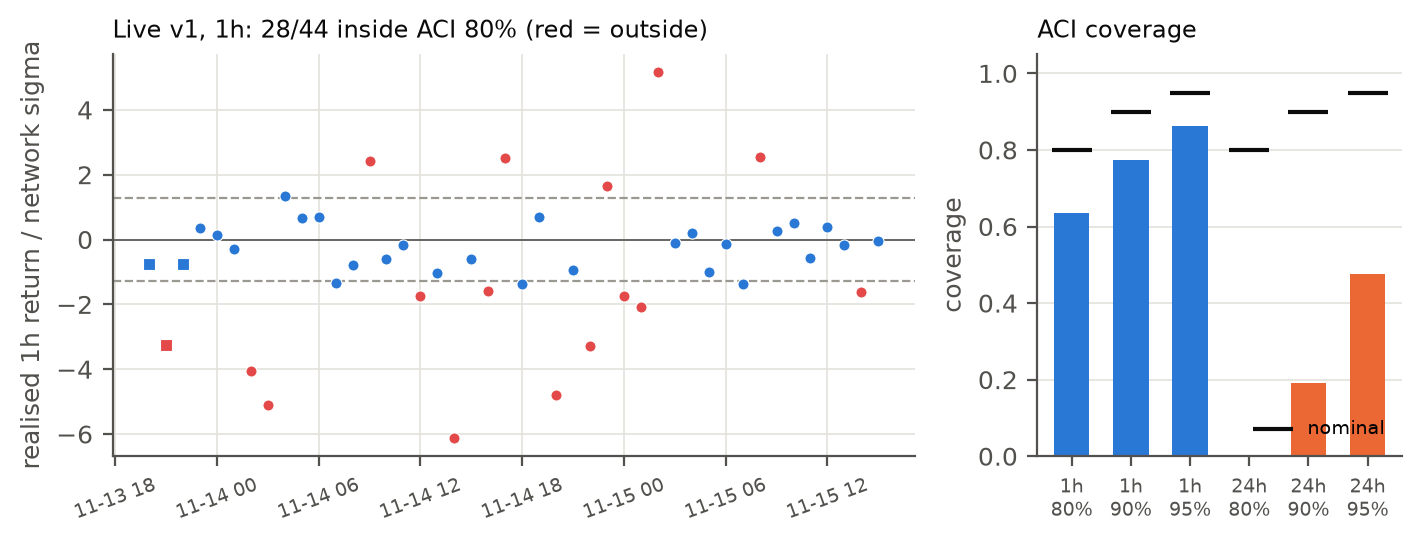
\includegraphics[width=0.95\textwidth]{figures/live_v1_scores.png}
\caption{Forward record of the live network v1 from \protect\path{data/journal/live_nn/scores.jsonl} (2026-11-13 to 2026-11-15). Left: realised 1-hour return in units of the network's sigma; the dashed lines are $\pm 1.28$. Right: ACI coverage by horizon and level. The 24-hour windows overlap and cover essentially one crash day.}
\label{fig:livescores}
\end{figure}

\paragraph{The dashboard and brain map.} A local read-only dashboard (\protect\path{src/ai_trader/livedash/}, \protect\path{research/live/dashboard/}) shows the live price inside the network's nested bands, the 24-hour cone, the field's touch probabilities, the regime-and-players strip and Claude's band (Figure~\ref{fig:dash}). The brain map re-runs the frozen network every tick with five of its 19 inputs rebuilt from the partial hour (pre-declared as \hyp{H-BR1}, an intra-hour nowcast) and draws the edges, latents and quantile heads as they change. Neither feeds any decision.

\begin{figure}[t]
\centering
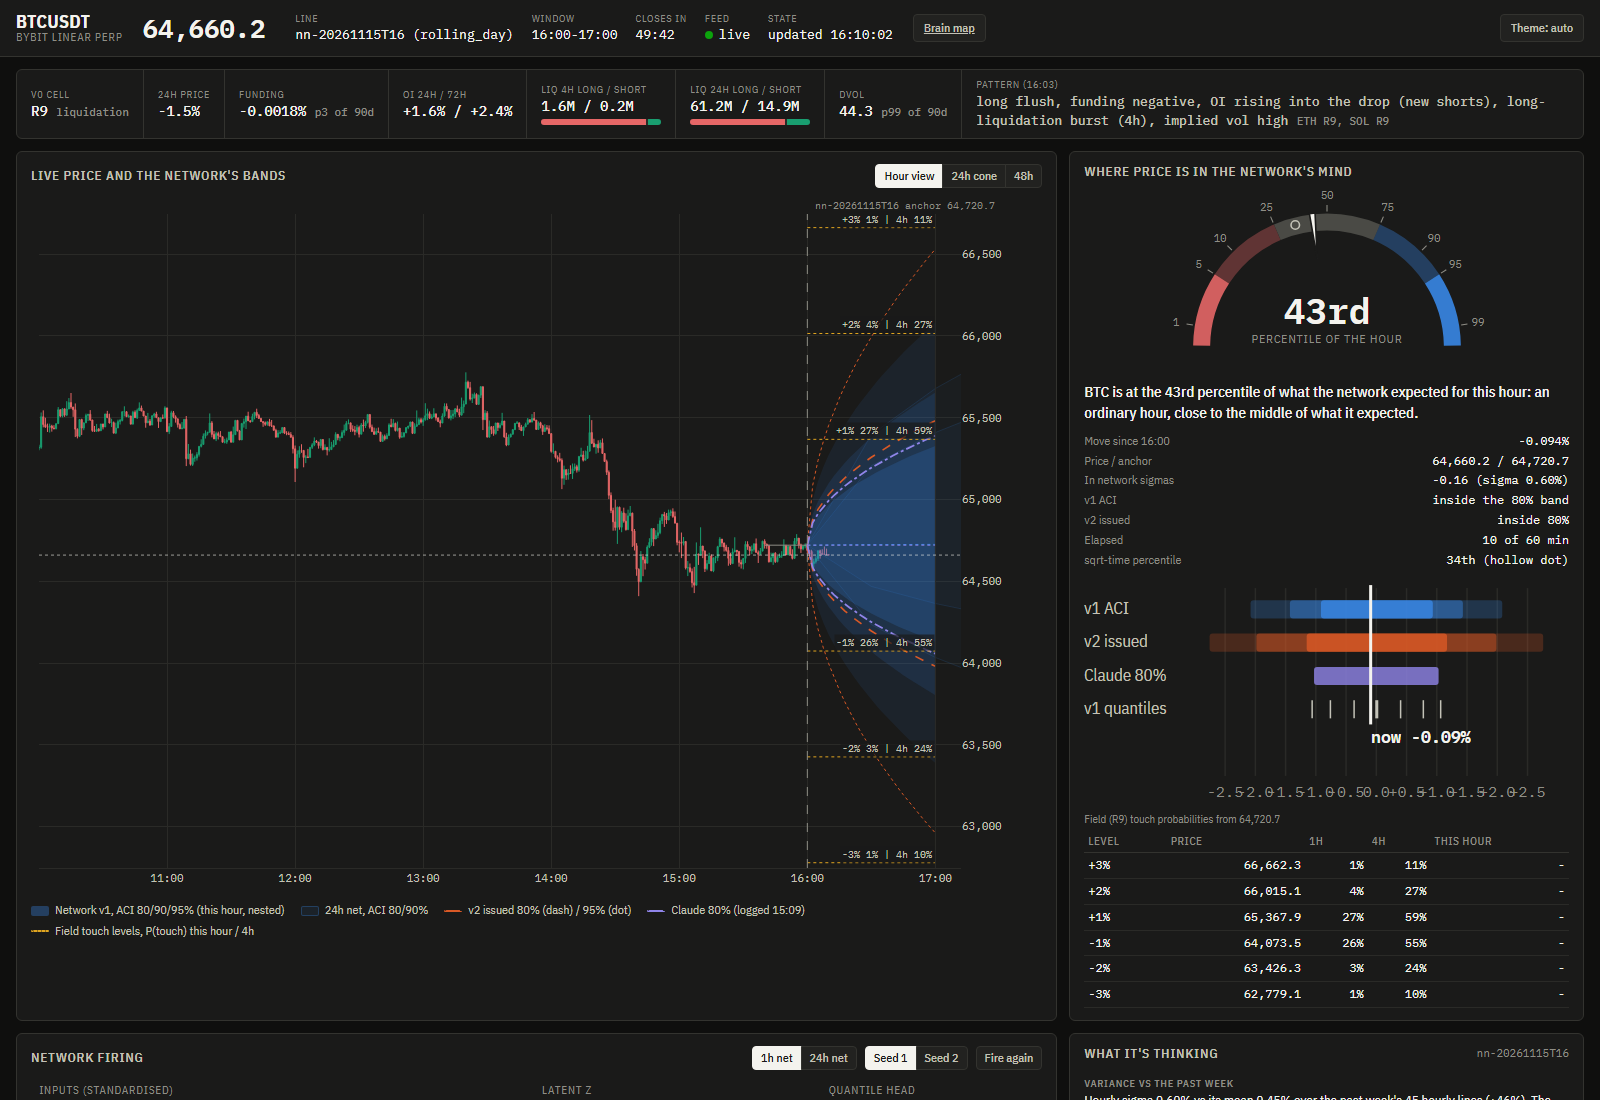
\includegraphics[width=0.98\textwidth]{figures/dashboard.png}\\[0.4em]
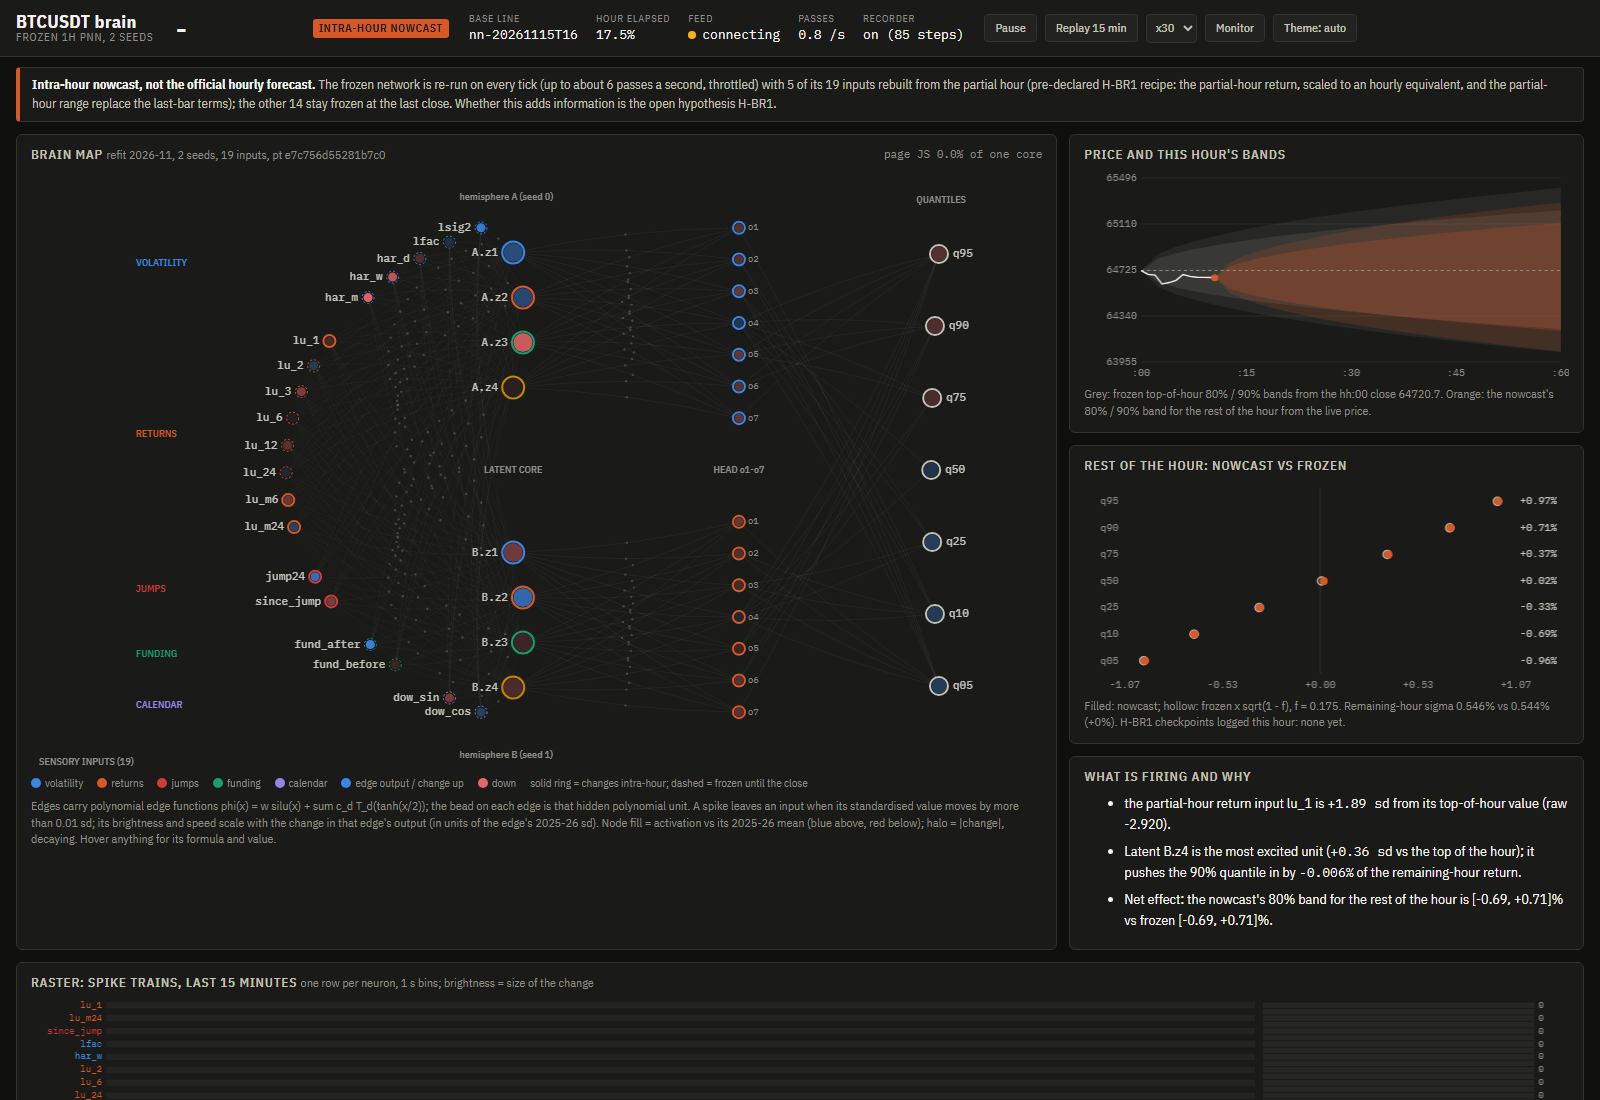
\includegraphics[width=0.98\textwidth]{figures/brain_map.png}
\caption{Screenshots of the local dashboard (top) and the brain map (bottom), captured headless on 2026-11-15 at about 16:10 UTC. The dashboard shows BTC inside the network's ACI bands, the 24-hour cone, the v2.1 and Claude bands and the field touch table; the brain map shows the two seeds (hemispheres) of the 1-hour network, its 19 inputs, 8 latent units and 7 quantile heads.}
\label{fig:dash}
\end{figure}

\paragraph{Regime and players.} The players block (\protect\path{src/ai_trader/live/players.py}) reports, point in time, the v0 regime cell, funding and its 90-day percentile, open interest changes over 24 and 72 hours, liquidations by side over 4 and 24 hours, and Deribit DVOL with its percentile, and turns them into one sentence from fixed rules. On 2026-11-15 at 16:03 UTC it read, for BTC: R9 liquidation, $-1.5\%$ over 24 hours, funding negative (3rd percentile), open interest rising into the drop (new shorts), a long-liquidation burst, DVOL at its 99th percentile. It is information only and changes no forecast.

\paragraph{The paper decision book.} Every four hours the harness prepares a session: it advances the persistent paper book, builds candidates from the two validated sleeves only (\texttt{shock\_regime} and \texttt{trend\_4h}), applies the bias gate and writes a short packet ($\le$ 120 lines, $\le$ 8 rules) for Claude. Claude answers take or skip for every candidate, with a reason and an optional bounded tilt in log-odds; the validator refuses any field that could steer size, stop, target, price or limits, and refuses answers after a 30-minute deadline. The takes go as intents through the Rust risk engine into the paper book, and the scorecard compares the AI book with RULE (every non-blocked candidate), RANDOM (same number of picks) and ALL on the same candidates. The first session with candidates (S20261115-0409) offered three shock-reversal shorts after a $+4.4\sigma$ Sunday up-shock in the R9 cell; Claude took ETH (net E[R] $+0.142$\,R, reward-to-risk 4.88, target probability 0.22, stop 0.62 sigma) and skipped BTC and SOL as the same bet. The pegged limit filled at 1,811.94, the trade reached $+1.49$\,R, and a Sunday squeeze then took it through the stop: $-1.28$\,R after costs. With a 22\% target probability a loss was the likely outcome; the diary records, as an observation for a later registered test, that a stop below about one hourly sigma in an R9 whipsaw tape looks fragile.

\paragraph{The live desk.} On 2026-11-15 the operator authorised a small live desk on Bybit USDT perps under hard limits that live in the Rust risk engine and in exchange-side stops, not in prompts (\texttt{live\_small} in \protect\path{config/risk.yaml}; \protect\path{crates/at-risk/src/live.rs}): at most \$2 loss per trade at the stop including fees and stop slippage, at most 20 entries per UTC day, a \$10 daily loss stop (realised plus open), at most 3 open positions and 2 in the same direction, \$400 gross notional, notional tiers of \$50 to \$200 by liquidity, PostOnly entries pegged to the touch, a minimum net expected value of 0.10\,R, correlated tokens treated as one bet, and manual approval by the operator for the first 5 live trades. The operator's numbers are compiled into the engine as ceilings, and a configuration looser than them is refused at load. \hyp{H-LT1} (positive net expectancy over $\ge$ 100 closed trades) and \hyp{H-LT2} (live fills match the paper fill model) were registered before any live order. At the time of writing no live trade had been made, and the honest state given to the operator was ``no validated edge yet''.

\FloatBarrier
%=====================================================================================================
\section{How we expect to make P\&L}
%=====================================================================================================

The research record does not contain a large, validated directional edge, and it would be dishonest to present the system as if it did. The expected sources of P\&L are small and specific.

\paragraph{Small validated edges.} (i) \emph{Shock fades in volatile cells and shock continuation in calm ones} (\hyp{H-S2}, forward-supported once; the paper sleeve \texttt{shock\_regime}); this is graded B/C and its own forward test (\hyp{H-S3}) has not decided yet. (ii) \emph{Limit entries at the touch}: $+0.010$\,R per signal, more for tight-stop sleeves ($+0.016$\,R for \texttt{shock\_regime}). This is a cost saving, not alpha. (iii) \emph{Volatility-aware stops and targets}: sizing on the unshrunk risk sigma, using log-HAR $\times$ weekday for expectations, jump-aware first-passage probabilities for brackets (\hyp{H-JD4}), and leaving room in exits because trend profits come from rare large days. These do not create edge; they stop a correct idea from being killed by noise or mis-sized. (iv) \emph{Avoiding known losers}: the 63 avoid-rules encode tested failures (fading 2$\sigma$ hourly moves, buying liquidation flushes, tight market making, mean reversion in trend cells, scaling out after extreme profits, trading direction from levels or weekends). The value of not trading these is real, but it is a reduction of losses relative to a naive trader, not a profit.

\paragraph{The LLM as filter and interpreter.} Claude's role is to filter candidates the deterministic layer has already passed, and to interpret context the rules cannot encode (an event, a regime transition, correlated candidates being the same bet). It cannot add size or remove a stop. Whether this filter adds value is exactly \hyp{H-AI1} (AI book minus RULE and minus RANDOM, both with $t>2$ over at least 60 closed AI trades; prior 0.20) and \hyp{H-AI2} (skipped candidates have lower mean R than taken ones over at least 100 resolved candidates). Because the baselines trade the same candidates in the same market, the paired difference has much lower variance than raw P\&L. Shadow outcomes for every ranked candidate add further data per session.

\paragraph{The cost model.} Crypto perps on this account pay 2\,bp maker and 5.5\,bp taker; the research default is 7.5\,bp per side. A pegged entry costs the maker fee plus about 1.3\,bp of adverse price (\hyp{H-EXE1}), so a pegged round trip with a taker stop is modelled at about 10.8\,bp instead of 15\,bp. The live profile adds a stop-exit slippage budget by liquidity tier (10, 25 and 60\,bp) inside the \$2 worst case, and refuses entries whose net expected value after these costs is below 0.10\,R.

\paragraph{Why the expectancy is uncertain.} Three reasons. First, the edges that survived are small relative to the noise: with a per-trade standard deviation near 1.2\,R, detecting a mean edge of 0.20\,R at $t\approx 2$ needs about 144 trades, and 0.10\,R needs about 576 (\protect\path{docs/PLAN.md}, \S5); at the live desk's pace that is weeks to months. Second, the holdout is short (about 135 days) and covers few regimes, and the trend edge that looked positive before the cutoff is negative after it. Third, every result is conditional on costs that a small account cannot reduce, and the paper fill model is itself a hypothesis (\hyp{H-LT2}).

\paragraph{What would falsify it.} The system's trading premise is falsified if \hyp{H-AI1} fails (Claude's selections do not beat RULE and RANDOM on the same candidates) or if \hyp{H-LT1} fails (mean net R per closed live trade is not positive with its 95\% CI above zero over at least 100 trades). Both had priors of 0.20 when registered, which, after the calibration of Section~3, is if anything generous. A failure of \hyp{H-LT2} would mean the paper record is not a valid stand-in for live trading.

%=====================================================================================================
\section{Advantages and disadvantages of each system}
%=====================================================================================================

\begin{table}[h]
\centering\small
\begin{tabularx}{\textwidth}{@{}p{3.0cm} L L@{}}
\toprule
System & Biggest advantage & Biggest disadvantage \\
\midrule
Point-in-time lake and collectors & Look-ahead is prevented by schema (\texttt{known\_ts}), not by convention; cheap (no server, 30\,GB budget) & Collectors die with their owning session or a sleeping machine; outages left gaps (43\% of symbol-minutes lost in one study) \\
Rust risk engine & Size, caps and stops are deterministic, tested and outside the LLM's reach; live ceilings fail closed & Conservative gates block most candidates (the EV gate first blocked every one), so evidence accrues slowly \\
Research protocol and registry & Pre-registration and the cutoff split expose optimism (22\% hit rate vs 0.44 priors) & Slow, and the holdout is short; most early verdicts are honestly ``inconclusive'' \\
Rules and playbook & The record compressed into 188 graded, traceable rules and short cards & Many rules are grade C; most say what \emph{not} to do, not what to do \\
Volatility models (log-HAR, hour-of-week, ML) & Large, stable gains in both segments; the robust core of the system & Forecast variance, not direction; they improve risk, not returns \\
Probability field & Interpretable equations for variance and jumps; stable coefficients & Its gain over log-HAR is the hour-of-week profile; no drift signal \\
PNN v1 / v2.1 live networks & Calibrated quantiles at 1\,h, conformal bands, interpretable edges & Polynomial edges add nothing over an MLP; live 24\,h bands under-covered in the first crash \\
Cross-sectional v3 & Best 1\,h vol forecasts across all 23 tokens & Ranking skill is mostly low volatility and loses after costs \\
\texttt{at-match} and the OB generator & Exact Bybit-semantics replay of real books and our own quoting code & Generated books miss signed-flow memory and cannot train or rank strategies \\
Market-making replay & Showed cheaply why live MM loses (1\,s adverse selection) & No positive configuration found after fees \\
vecopen & Strict phases, tamper-evident registry, independent leak audit & G2 not yet run; waits on CFD data \\
Paper decision harness & Forward, paired, deadline-bound evaluation of Claude's choices & Few candidates per week; one trade so far ($-1.28$\,R) \\
Live desk (\texttt{live\_small}) & Hard limits in code; real fills and costs; first 5 trades approved by the operator & No validated edge yet; tiny sizes make fees dominant \\
Dashboard and brain map & Makes the models' state legible to the operator and to Claude & Descriptive only; risk of over-reading pictures \\
\bottomrule
\end{tabularx}
\caption{The single biggest advantage and disadvantage of each component.}
\label{tab:proscons}
\end{table}

%=====================================================================================================
\section{Lessons and mistakes}
\label{sec:lessons}
%=====================================================================================================

The diary (\protect\path{research/diary/}) records mistakes as they happen and is never edited; this section summarises them.

\paragraph{Operations: timers, sleep and processes.} Registering Windows scheduled tasks was refused by the permission system and left to the operator (2026-11-07, 2026-11-08). The collector and the updater died with the session that owned them, leaving a gap from 2026-11-11 02:46 to 2026-11-12 03:45 UTC that was found only when the frozen volatility model flagged every symbol as stale. On 2026-11-12 the machine slept for about three hours; agents and jobs died, and the NVDA quoter's resting quotes stayed live and unmanaged. On 2026-11-14 scheduled reminders inside the session never fired, so no Claude forecasts exist for 01:00--11:00 UTC; the schedule was replaced by a monitor ticker and the gap was not back-filled.

\paragraph{Agents killing processes.} On 2026-11-08 the quoter died with the signature of a forced kill after the operator had rejected a flatten, and the wrapper then market-flattened at a cost of a few cents; the operator's rule since then is never to stop or flatten a live run unless a predefined rule fires or the operator asks, and the wrapper now restarts with \texttt{--adopt}. On 2026-11-09 a task stop did not kill the wrapper loop, which restarted the quoter (kill the wrapper first). On 2026-11-14 two replay days were lost because another agent rebuilt the shared binary mid-run (replays now use a private copy). On 2026-11-15 an agent killed 14 watcher processes it did not own by pattern-matching a path; the lesson is to kill only by one's own recorded PID.

\paragraph{GDELT.} GDELT returned HTTP 429 after a few test calls on 2026-11-08 and again from 2026-11-13 21:31 UTC, leaving 3 of 20 news series. The study refused to record verdicts on partial data; the operator dropped GDELT, \hyp{H-NEWS1/2} were recorded as inconclusive (not run), and \hyp{H-NEWS3/4} were registered on sources whose history can be downloaded. A FinancialJuice feed was stopped at the access check because its terms forbid automated collection.

\paragraph{Holdout glimpses.} The protocol reads the holdout once per hypothesis, and several glimpses were disclosed rather than hidden. The shock-reversal pattern \hyp{H-S3} was first seen in the holdout, so it is testable only on data after 2026-11-08. A debug run showed outcome numbers before a full flow study; no threshold was changed. A simulator design was iterated about six times while looking at test facts of five symbols; this was disclosed as a bias toward support (the hypothesis was contradicted anyway). In vecopen a builder printed two rows of a file that later became holdout, and a superseded run printed counts from which a crude placebo touch rate could be derived; the counts were removed, the run repeated, nothing retuned, and the reviewers never saw them. \hyp{H-LIVE2} was amended before any data existed because its first test had no fair null.

\paragraph{Corrections.} The operator corrected the system twice in ways that changed its rules: the never-stop, never-flatten rule above, and the observation on 2026-11-12 that a bullish lean with a positive inventory target in the NVDA market maker was a directional bet that was crystallising losses; live market making was stopped and the project went research-only until the live desk was authorised on 2026-11-15. Claude had to correct itself as well: on 2026-11-14 it had told the operator that the short deep-ITM put barely changes vega, and the Greeks showed it cuts vega by about 74\%. Other wrong claims were corrected in the record: that Bybit TradFi perps freeze on weekends (they trade 24/7 at 0.1--0.15$\times$ weekday turnover); a CPI print reported as 4.0\% that was 3.7\% because of a missing month; and an untested proxy briefly ranked as the top alpha. Bugs found by tests included an \texttt{Int8} overflow in session labels, a full-sample median in a weekend filter (look-ahead), an exchange clock 0.3\,s ahead that put \texttt{known\_ts} before the candle end, a market-maker sigma that always fell back to its floor (\texttt{sigma\_last} in \texttt{mm.rs}), and several NaN-versus-null leaks.

\paragraph{Overfitting traps avoided.} A prior project's champion rule (Sharpe 0.8, chosen from 300--500 configurations that reused the out-of-sample half) had Sharpe $-0.12$ on unseen data; that experience produced the protocol's rules. In this project the best trend variant's deflated Sharpe was 0.72 against a 0.95 bar, walk-forward selection lost to the plain ensemble, per-symbol parameter selection had PBO 0.44--0.65, the volatility-break filter had DSR 0.22 and PBO 0.84, mined discovery lists were frozen with a hash before confirmation, and a market-making PBO of 0.00 was explicitly flagged as uninformative because most variants were dominated.

%=====================================================================================================
\section{Conclusion and next steps}
%=====================================================================================================

Nine days of work produced a point-in-time data platform, a Rust risk and execution path, a research protocol that measured its own optimism, a large body of mostly negative but well-documented results, and a set of frozen, calibrated volatility models now running live. The central empirical finding is consistent across every programme: volatility is forecastable and largely calendar-driven, direction is not forecastable from the inputs tried, and the only measured trading improvements are small execution and risk-management gains. The question the project was built to answer, whether an LLM adds value as a filter and interpreter on top of such a deterministic layer, has not been answered yet; it is now set up to be answered cleanly.

Next steps follow from the registered tests: accrue the paper book to the \hyp{H-AI1} sample, the Claude forecasts to the \hyp{H-LIVE1} sample and the live desk to the \hyp{H-LT1/LT2} samples without changing pinned versions mid-record; evaluate v2.1 against v1 on live lines only; run vecopen gate G2 once the CFD history exists; finish the forward tests of the calendar and volatility rules (\hyp{H-VM6}, \hyp{H-DS4}, \hyp{H-NN10}); and keep recording failures.

\FloatBarrier
\bibliographystyle{plainnat}
\bibliography{ai_trader_paper}

\appendix
%=====================================================================================================
\section{Reproducibility}
%=====================================================================================================

\paragraph{Commands.} All commands run from the repository root.
{\small
\begin{verbatim}
cargo test --workspace                           # Rust tests
cargo clippy --workspace --all-targets           # lint
uv run pytest                                    # Python tests
target/debug/atx check                           # connectivity
uv run python scripts/run_research.py            # playbook and verdicts
uv run python -m ai_trader.research.rules        # validate rules, write RULES.md
uv run python scripts/knowledge_book.py --date YYYY-MM-DD
PYTHONIOENCODING=utf-8 uv run --extra ml python scripts/live_nn.py --dry-run
PYTHONIOENCODING=utf-8 uv run python scripts/live_score.py          # H-LIVE running stats
uv run --extra vecopen python -m vecopen verify                     # vecopen registry chain
PYTHONIOENCODING=utf-8 uv run --extra viz python paper/make_figures.py
\end{verbatim}
}
The figures new to this paper are produced by \protect\path{paper/make_figures.py}, which reads the registry, the results file and the live score journal and copies the reused figures unchanged from \protect\path{research/figures/}.

\paragraph{Frozen models.} SHA-256 of the frozen artefacts read by the live system, computed on 2026-11-15.
{\footnotesize
\begin{longtable}{@{}p{5.5cm}p{10.3cm}@{}}
\toprule
File & SHA-256 \\
\midrule
\protect\path{data/models/pnn/wf_1h/2026-11.pt} & \texttt{e7c756d55281b7c0a219e3a6cbbf517d3791490bbf325370ef77220118781a44} \\
\protect\path{data/models/pnn/wf_1d/2026-11.pt} & \texttt{0f22c2a234114985b468544c1da3243705d3518b754b763a58bcd9c3b973deea} \\
\protect\path{data/models/pnn/frozen_1h.json} & \texttt{56ae1e478f50efbd643fe0f6c90c2ead734405397cb6a47e7f6e59b1a5f41627} \\
\protect\path{data/models/pnn/frozen_1d.json} & \texttt{76037c1f8f01223c08b7186966faba8bfec4c2c685e9b20c7e2758993f79bedc} \\
\protect\path{data/models/xs_v3/frozen/spec.json} & \texttt{cfb9ba3579e9a3b45f5e8a8e941aa6ecbe94956e5273b9336681a0cfed1f0ed2} \\
\protect\path{data/models/xs_v3/frozen/v3_seed0.pt} & \texttt{94bcf0ae7897c2c2d9c7c5df69483e887039fc17f9d5b5ba335b19f03b4c9a89} \\
\protect\path{data/models/xs_v3/frozen/v3_seed1.pt} & \texttt{985fd325147f0853da5d5ccf16b4d6e5b4bd6ea29199d007e582df66529c5c79} \\
\protect\path{data/models/xs_v3/frozen/v3_seed2.pt} & \texttt{471b0b4d5a5281ac77276c49d2b7dd01e78511529977b6cae41d47adcc2e502a} \\
\protect\path{data/models/field/btc_field_cutoff_2026-07-01.json} & \texttt{87fd08998d9c60a093a8be04b5d392df9ab59f82ca97dc77dc19f564b51fb95a} \\
\protect\path{data/models/field/btc_field_2026-11-13.json} & \texttt{d54a24a3fdb54d532dec84c996e44a763e3eb5f62f5fc5f593d8ca8520de9a41} \\
\protect\path{config/live_nn_v2.yaml} (file) & \texttt{3dc6599341e713f28387945149e6f4e96a46dcb86264e4303d7352f829330160} \\
\bottomrule
\end{longtable}
}
\noindent The v2.1 lines log a hash of the \emph{parsed} configuration (\texttt{2d4ba801a6363fe9}); vecopen's frozen baseline configuration has SHA-256 \texttt{9e78f831b0e95c6824529485628b0c1777733db5374f6e0f6163894f0c2ae14a}. The pinned decision model is \texttt{claude-opus-5-5}; the forecast prompt is \texttt{live\_claude.v2} and the decision packet \texttt{compact-2} (harness \texttt{decision\_session.v1}).

\end{document}
